\documentclass[11pt]{article}
\usepackage[T1]{fontenc}
\usepackage[utf8]{inputenc}
\usepackage{lmodern}
\usepackage[a4paper,margin=2.2cm]{geometry}
\usepackage{amsmath,amssymb,mathtools}
\usepackage{booktabs,tabularx,xltabular,array}
\usepackage{enumitem}
\usepackage[dvipsnames]{xcolor}
\usepackage{tikz}
\usetikzlibrary{arrows.meta,positioning,calc}
\usepackage{microtype}
\usepackage[hyphens]{url}
\usepackage[colorlinks=true,linkcolor=blue!50!black,urlcolor=blue!50!black]{hyperref}
\usepackage[most]{tcolorbox}

\setlength{\emergencystretch}{3em}
\setlist{nosep,leftmargin=1.4em}
\setlength{\parindent}{0pt}
\setlength{\parskip}{0.45em}
\renewcommand{\arraystretch}{1.15}

\definecolor{good}{HTML}{2E7D4F}
\definecolor{warn}{HTML}{B8730A}
\definecolor{bad}{HTML}{B5403A}
\definecolor{steel}{HTML}{2F4B6E}
\definecolor{gA}{HTML}{2F4B6E}
\definecolor{gB}{HTML}{2E7D4F}
\definecolor{gC}{HTML}{8A4F9E}
\definecolor{gD}{HTML}{B8730A}

\def\UrlBreaks{\do\/\do\_\do\.\do\-\do\:}
\DeclareUrlCommand\code{\urlstyle{tt}}

\newcommand{\stbuilt}{\textcolor{good}{\textbf{Built}}}
\newcommand{\stpartial}{\textcolor{warn}{\textbf{Partial}}}
\newcommand{\stnot}{\textcolor{bad}{\textbf{Not built}}}
\newcommand{\GA}{\textcolor{gA}{\textbf{G1}}}
\newcommand{\GB}{\textcolor{gB}{\textbf{G2}}}
\newcommand{\GC}{\textcolor{gC}{\textbf{G3}}}
\newcommand{\GD}{\textcolor{gD}{\textbf{G4}}}
\newcommand{\fld}[1]{\par\medskip\noindent\textbf{\textcolor{steel}{#1}}\par\nopagebreak}
\newcommand{\intu}[1]{\par\noindent{\small\textit{Intuition.} #1}\par}
\newcommand{\sym}[1]{\par\noindent{\small\textit{Symbols.} #1}\par}
\newtcolorbox{flagbox}{colback=bad!6,colframe=bad,boxrule=0.6pt,arc=1pt,left=4pt,right=4pt,top=3pt,bottom=3pt}
\newtcolorbox{notebox}{colback=steel!5,colframe=steel!60,boxrule=0.5pt,arc=1pt,left=4pt,right=4pt,top=3pt,bottom=3pt}
\newtcolorbox{algobox}{colback=white,colframe=steel!50,boxrule=0.5pt,arc=1pt,left=5pt,right=5pt,top=3pt,bottom=3pt,breakable}

\title{HY Analyst: one combined framework\\[2pt]
\large Four groups of method, one pipeline, one expected alpha}
\author{FundamentalQuantmental repository}
\date{22 October 2026}

\begin{document}
\maketitle
\thispagestyle{empty}
\section*{Summary}
\addcontentsline{toc}{section}{Summary}

\begin{enumerate}[leftmargin=1.6em,itemsep=0.3em]
\item This document defines one framework for one analyst. It merges four groups of method into a single pipeline of fifteen steps, plus a size calibration step.
\item The four groups are: \GA{} the core process (Gatto's seven steps, the methodology, the framework rules, and the relative value PDF); \GB{} the methods the code already runs; \GC{} seven credit skills, written for private loans and adapted here to public bonds; and \GD{} two books, Kricheff and Ganguin and Bilardello (S\&P).
\item The analyst loads data stamped with the date it became public, frames the business, cleans earnings, and measures liquidity, claims, covenants, and the gap between fixed charges and signed contracts (the two clocks).
\item The analyst then projects the issuer under five macro stories, values the firm and each bond's recovery, and finds the spread each bond should pay.
\item All of this becomes one number: expected alpha, the six-month return of a hedged long after default loss and cost. The weights are the user's: 40\% on the core process, 20\% on the two clocks, 18\% on the rest of the built methods, 17\% on the books and peers, and 5\% on the skills (which can only lower the number).
\item The code now charges default loss on the price paid, not on face value. In the gate, the row that turned spread into a default probability no longer votes. A breakeven-default row votes instead: the default rate at which the spread only pays for its loss.
\item The severe-case runway now funds committed capex, so it no longer hides the cash burn of growth commitments.
\item The size calibration is built. The backtest slope is 0.079 (standard error 0.054). That is not reliably above zero, so the number ranks issuers but does not size positions.
\item The decision against cash (S15) is built. It compares each bond with every other use of the same money, cash included, and names the position it would replace. Only this step may say ``buy''.
\item Real gaps remain. The claims, recovery and covenant work is only partly wired into the pipeline. Credit lines are untagged in the filings, so revolver capacity is missing. Gate rules G4, G5, G7, G8 and G9 are not built.
\end{enumerate}

\begin{notebox}
\textbf{What this means for you.} The ranking is usable; the sizes are not. Under the earlier weights CoreWeave showed a raw alpha of +145 bp a year after cost, and +11 bp after calibration. The new weights lean on the core rules and the clocks, where CoreWeave scores poorly, so its figure is likely to fall. Agent one is rerunning; read the new figures in the memo, not here.
\end{notebox}
\newpage
\section*{The single analyst pipeline}
\addcontentsline{toc}{section}{The single analyst pipeline}

\begin{center}
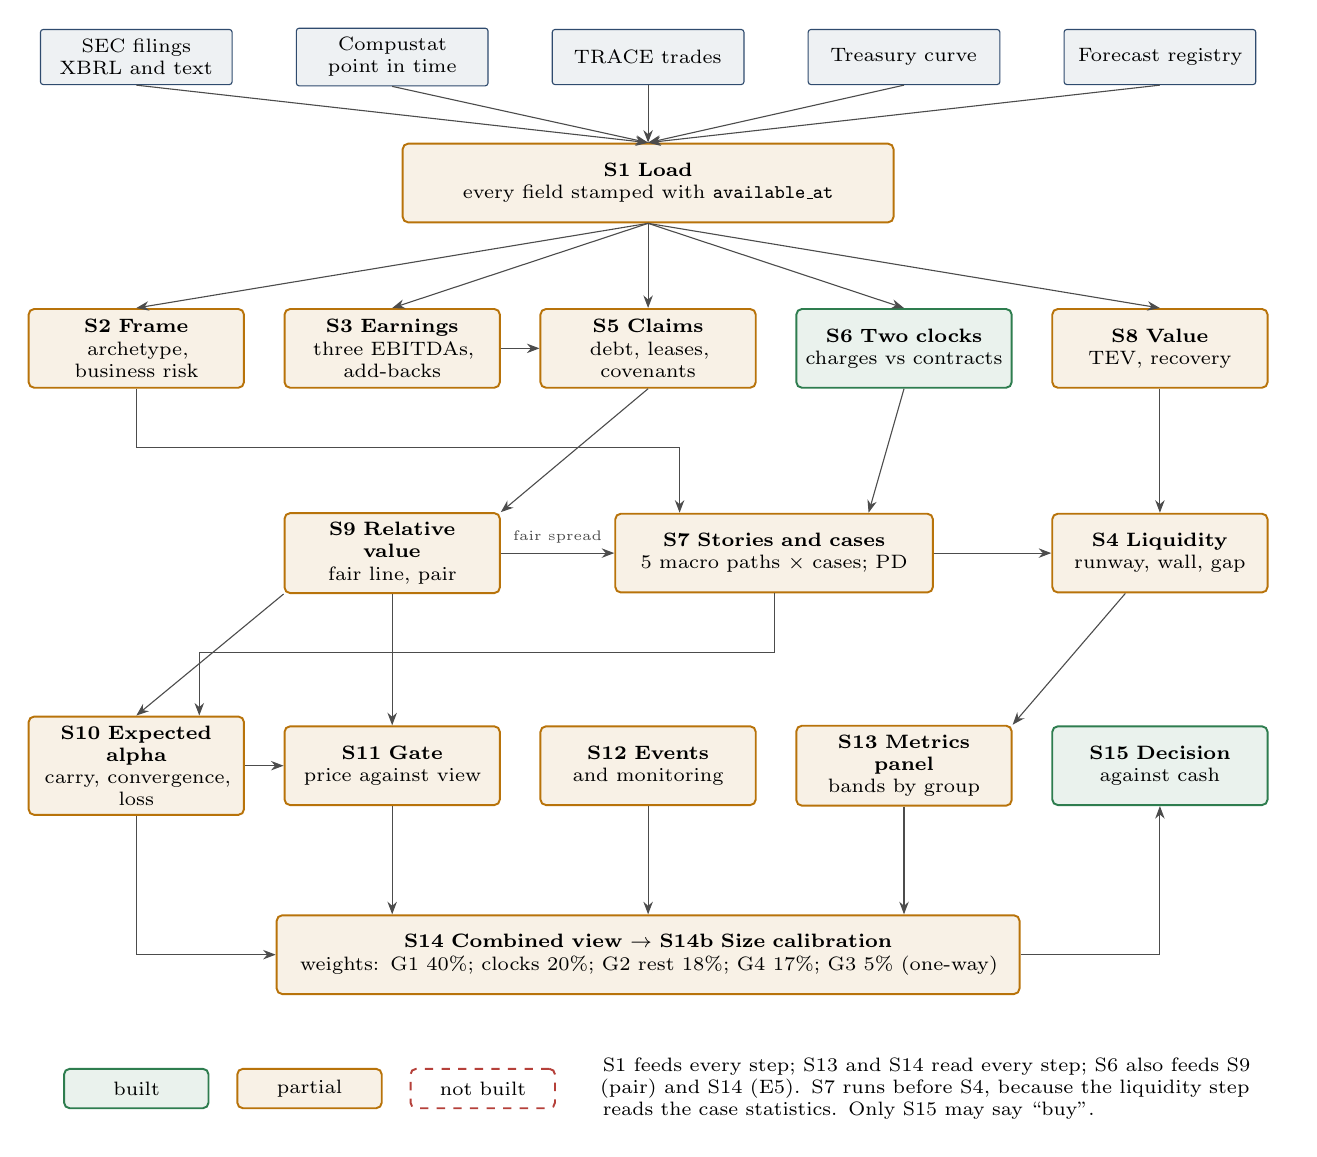
\begin{tikzpicture}[
  x=1cm,y=1cm,
  box/.style={draw,rounded corners=2pt,align=center,font=\scriptsize,minimum height=10mm,text width=25mm,line width=0.7pt,execute at begin node={\hyphenpenalty=10000\relax}},
  src/.style={draw=steel,fill=steel!8,rounded corners=1pt,align=center,font=\scriptsize,minimum height=7mm,text width=22mm},
  b/.style={box,draw=good,fill=good!10},
  p/.style={box,draw=warn,fill=warn!10},
  n/.style={box,draw=bad,fill=white,dashed},
  a/.style={-{Stealth[length=1.6mm]},thin,gray!60!black},
  lab/.style={font=\scriptsize\bfseries,text=steel,rotate=90,anchor=center}]
% sources
\node[src] (sx) at (0,0) {SEC filings\\XBRL and text};
\node[src] (sc) at (3.25,0) {Compustat\\point in time};
\node[src] (st) at (6.5,0) {TRACE trades};
\node[src] (su) at (9.75,0) {Treasury curve};
\node[src] (sf) at (13,0) {Forecast registry};
\node[p,text width=60mm] (s1) at (6.5,-1.6) {\textbf{S1 Load}\\every field stamped with \texttt{available\_at}};
\foreach \s in {sx,sc,st,su,sf} \draw[a] (\s.south) -- (s1.north);
% measure
\node[p] (s2) at (0,-3.7) {\textbf{S2 Frame}\\archetype, business risk};
\node[p] (s3) at (3.25,-3.7) {\textbf{S3 Earnings}\\three EBITDAs, add-backs};
\node[p] (s5) at (6.5,-3.7) {\textbf{S5 Claims}\\debt, leases, covenants};
\node[b] (s6) at (9.75,-3.7) {\textbf{S6 Two clocks}\\charges vs contracts};
\node[p] (s8) at (13,-3.7) {\textbf{S8 Value}\\TEV, recovery};
\foreach \s in {s2,s3,s5,s6,s8} \draw[a] (s1.south) -- (\s.north);
\draw[a] (s3) -- (s5);
% forecast and price
\node[p] (s9) at (3.25,-6.3) {\textbf{S9 Relative}\\\textbf{value}\\fair line, pair};
\node[p,text width=38mm] (s7) at (8.1,-6.3) {\textbf{S7 Stories and cases}\\5 macro paths $\times$ cases; PD};
\node[p] (s4) at (13,-6.3) {\textbf{S4 Liquidity}\\runway, wall, gap};
\draw[a] (s5.south) -- (s9.north east);
\draw[a] (s6.south) -- ($(s7.north)+(1.2,0)$);
\draw[a] (s9) -- node[above,font=\tiny]{fair spread} (s7);
\draw[a] (s2.south) -- ++(0,-0.75) -| ($(s7.north)+(-1.2,0)$);
\draw[a] (s7) -- (s4);
\draw[a] (s8) -- (s4);
% decide
\node[p] (s10) at (0,-9.0) {\textbf{S10 Expected}\\\textbf{alpha}\\carry, convergence,\\loss};
\node[p] (s11) at (3.25,-9.0) {\textbf{S11 Gate}\\price against view};
\node[p] (s12) at (6.5,-9.0) {\textbf{S12 Events}\\and monitoring};
\node[p] (s13) at (9.75,-9.0) {\textbf{S13 Metrics}\\\textbf{panel}\\bands by group};
\node[b] (s15) at (13,-9.0) {\textbf{S15 Decision}\\against cash};
\draw[a] (s9.south west) -- (s10.north);
\draw[a] (s7.south) -- ++(0,-0.75) -| ($(s10.north)+(0.8,0)$);
\draw[a] (s9) -- (s11);
\draw[a] (s10) -- (s11);
\draw[a] (s4) -- (s13.north east);
% combine
\node[p,text width=92mm] (s14) at (6.5,-11.4) {\textbf{S14 Combined view} $\rightarrow$ \textbf{S14b Size calibration}\\weights: G1 40\%; clocks 20\%; G2 rest 18\%; G4 17\%; G3 5\% (one-way)};
\draw[a] (s10.south) |- (s14.west);
\foreach \s in {s11,s12,s13} \draw[a] (\s.south) -- (s14.north -| \s.south);
\draw[a] (s14.east) -| (s15.south);
% legend
\node[b,text width=16mm,minimum height=5mm] at (0,-13.1) {built};
\node[p,text width=16mm,minimum height=5mm] at (2.2,-13.1) {partial};
\node[n,text width=16mm,minimum height=5mm] at (4.4,-13.1) {not built};
\node[font=\scriptsize,anchor=west,text width=86mm] at (5.8,-13.1) {S1 feeds every step; S13 and S14 read every step; S6 also feeds S9 (pair) and S14 (E5). S7 runs before S4, because the liquidity step reads the case statistics. Only S15 may say ``buy''.};
\end{tikzpicture}
\end{center}

\textbf{How to read it.} One analyst runs every step, in order, for each issuer. The four groups do not run as separate pipelines. Each group adds rules, metrics or checks to the same steps. The last three steps turn the results into a decision:
\begin{itemize}\itemsep0pt
\item S14 combines all the estimates into one number, the expected alpha. Expected alpha is the six-month return of a hedged long position after default loss and the cost to buy and sell.
\item S14b scales that number down to the size that history supports.
\item S15 compares the bond with every other use of the same money, cash included.
\end{itemize}
\newpage
\section*{The four groups}
\addcontentsline{toc}{section}{The four groups}

{\footnotesize
\begin{xltabular}{\linewidth}{@{}>{\raggedright\arraybackslash}p{13mm}>{\raggedright\arraybackslash}p{42mm}>{\raggedright\arraybackslash}X>{\raggedright\arraybackslash}p{30mm}@{}}
\toprule
Group & Sources & What it brings to the one framework & Role in the score \\
\midrule
\endhead
\GA{} Core process & Gatto, \emph{The Credit Investor's Handbook} (2023); \code{docs/methodology.md}; \code{docs/framework.md} F1--F13; relative value PDF via \code{research/hyrv_extract.md} and \code{research/hyrv_mapping.md} & The order of the steps; the rules (point in time, two views, claims sizing, the gate); the formulas; the PDF's decision against cash and its strict rules on PD, loss and averaging & 40\% of the score (E4, E7--E10); the loss on price; the gate; size calibration; the decision \\
\GB{} Built methods & Two clocks (M4.7, Radhakrishnan card); fair line and pair (\code{scripts/rv_pair.py}); stories and forecast sources (\code{hy/macro.py}, \code{hy/forecasts.py}, eleven forecast cards); cases and alpha (\code{scripts/scenarios.py}, \code{hy/alpha.py}); F9 gate, F8 panel, combined view (\code{scripts/process.py}); the backtest (\code{hy/backtest.py}) & Working code on real data for eight issuers; the only measured evidence (the backtest) & Two clocks (E5): 20\%; the rest (E0--E3, E6): 18\% \\
\GC{} Skills & \code{hy-model-standards}; \code{credit-model-standards}; \code{credit-memo-standards}; \code{ebitda-addback-treatment}; \code{covenant-compliance}; \code{borrower-monitoring}; \code{quarterly-package-extraction} & Practitioner rules: three EBITDAs, add-back push-back thresholds, FCF cross-check, covenant headroom and trajectory, watchlist tiers, debt bridges. Written for private loans; where a rule does not transfer to public bonds, the step says so & 5\%, one-way (E11); E7 is one-way but counted in G1 \\
\GD{} Books and peers & Kricheff, \emph{A Pragmatist's Guide to Leveraged Finance}; Ganguin and Bilardello, \emph{Standard \& Poor's Fundamentals of Corporate Credit Analysis} (2005); Dynkin et al., \emph{Systematic Investing in Credit} (2021), ch.~13--14 & Kricheff: cash-flow underwriting, spread per turn and its trap, covenant capacity, event pro formas, recovery timing. S\&P: business risk grading, analytical adjustments (leases, pensions), ratio medians by rating, stress and default cases, recovery method. Dynkin et al.: excess spread to peers (ESP) and SPiDER & 17\%: E12 (S\&P score gap), E13 (spread per turn), E14 (ESP), E15 (SPiDER) \\
\bottomrule
\end{xltabular}
}

\textbf{Out of scope.} The other reading-list books are not available locally and add nothing here: Fridson and Alvarez; Moyer; Altman, Hotchkiss and Wang; Whitman and Diz; Lando; Duffie and Singleton; Marks. The seed papers are dropped.

\textbf{Source notes.} The Kricheff markdown lost the contents of every table; only numbers quoted in the text survive. Both books contain a few arithmetic slips (Kricheff Ch.~10 and 16; S\&P Ch.~9, 10 and 11); this document does not copy them. Book page numbers are not used; chapters are.

\textbf{How to read a step.} Each step gives, in order: purpose; what each group contributes; one merged algorithm; metrics with symbols and intuition; bands; inputs (data, documents, analyst); outputs; where groups disagree and which rule wins; the settling test; status in the code; and a short CoreWeave (CRWV) example from \code{data/raw/process/CRWV.json}. Status: \stbuilt{} means the code computes the step's main output on real data; \stpartial{} means part of it, and the step names what is missing; \stnot{} means no code runs it. Labels: ``M4.3'' is a methodology section; ``F5'' a framework rule; ``E31'', ``R49'', ``P11'', ``U17'' are relative value PDF items; ``C'', ``K'' and ``B'' are rows of the conflicts register (Section~\ref{sec:conflicts}).

% Two pages per group. Charts: scripts/group_pages.py writes fig_bucket_*.tex from data/raw/process/<T>.json.
% Values are bucket alpha in bp a year before cost, from the run of 22 October 2026 (user bucket weights, second revision).

\newpage
\section*{\textcolor{gA}{G1} Core process}
\addcontentsline{toc}{section}{G1 Core process}

\begin{notebox}
\textbf{In one line.} G1 sets the order of the steps and the rules that every number must obey. It carries 40\% of the score, the largest share.
\end{notebox}

\fld{What it is}
G1 is the base process and the rulebook. It has four sources:
\begin{itemize}
\item Gatto, \emph{The Credit Investor's Handbook} (Wiley, 2023). Its seven steps, Chapters 6 to 13, give the order of the analysis.
\item \code{docs/methodology.md}, sections M1 to M11. It gives the formulas: cases, recovery, fair spread, alpha and validation.
\item \code{docs/framework.md}, rules F1 to F13. It gives the rules: point in time, claims sizing, the gate and the memo.
\item The relative value PDF, read through \code{research/hyrv_extract.md} and \code{research/hyrv_mapping.md}. It adds the decision against cash and strict rules on default, loss and averages.
\end{itemize}

\fld{Why it is in the framework}
Without G1, the other groups have no common order and no common rules. G1 also holds the two hard stops. The S11 gate can block any call. Only S15 may say ``buy''.

\fld{What it adds at each step}
{\footnotesize
\begin{tabularx}{\linewidth}{@{}>{\raggedright\arraybackslash}p{24mm}>{\raggedright\arraybackslash}X@{}}
\toprule
Step & G1 contribution \\
\midrule
S1 Load & Every field carries \code{as_of} and \code{available_at}. A memo dated $t$ reads nothing released after $t$. TRACE prices are estimates, not quotes. \\
S2 Business & Gatto step 2: industry risks, strategy, management. F2: five lines and one archetype A1 to A8. \\
S3 Earnings & Gatto step 3a: remove one-off items. F3: keep three EBITDAs apart. Add-back classes C1 to C10. \\
S4 Liquidity & Gatto step 3b: liquidity, maturities, access to refinance. F4: effective liquidity, runway, the wall, the refinance score. \\
S5 Claims & Gatto steps 3c and 6: the capital structure table and the covenants. F5: size every claim, leases included. \\
S6 Clocks & M4.7: the formulas and five rules. Gatto has no such measure. \\
S7 Cases & Gatto step 4: base and downside cases. M5: the case engine under each macro path. \\
S8 Value & Gatto step 5: comparables, DCF, liquidation. M6 and F7: value, waterfall, recovery. \\
S9 Relative value & Gatto step 7: risk is PD times LGD. M7.2: the fair spread. \\
S10 Alpha & M7.5: carry, convergence, loss and cost. The PDF: reprice each path with default inside the cash flows. \\
S11 Gate & F9: rules G1 to G9. A wide spread never waives an open step. \\
S12 Events & M9 and F11: the event list and the playbooks. \\
S13 Metrics & F8: formula, unit, direction and bands for every metric. \\
S14b Size & M11: check every forecast against what happened. \\
S15 Decision & The PDF, Step 7: compare the bond with every other use of the money, cash included. \\
\bottomrule
\end{tabularx}
}

\newpage
\fld{Its estimates in the score}
G1 holds five estimates. They share its 40\%.\par
{\footnotesize
\begin{tabularx}{\linewidth}{@{}>{\raggedright\arraybackslash}p{8mm}>{\raggedright\arraybackslash}p{34mm}>{\raggedright\arraybackslash}X>{\raggedright\arraybackslash}p{12mm}@{}}
\toprule
ID & Estimate & How the code computes it & Weight \\
\midrule
E4 & Default the price assumes & $(PD^{\kappa} - PD^{fund})\,L^{def}$. The code shows it but does not count it until $\kappa$ is fitted (conflict C2). & 0\% \\
E7 & Earnings quality & Minus the count of F3, add-back and FCF-check flags. It can only lower the number. & 10.00\% \\
E8 & Liquidity and refinancing & F4 score on the likely path, plus wall cover (cap 3), plus one point if no funding gap. & 10.00\% \\
E9 & Market value check & Minus debt over market enterprise value. & 10.00\% \\
E10 & Excess over cash & $\mu/H$ from S15: the expected gain over cash, per year. & 10.00\% \\
\bottomrule
\end{tabularx}
}

\fld{What it says about the eight issuers}
\begin{center}
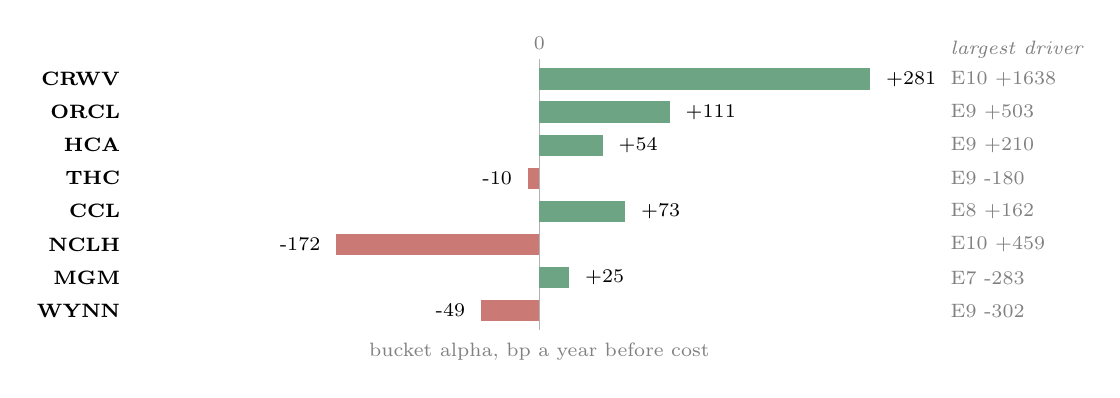
\begin{tikzpicture}[x=1cm,y=0.42cm,font=\scriptsize]
\draw[gray!60] (0,0.6) -- (0,-7.6);
\node[gray,anchor=south] at (0,0.6) {0};
\node[anchor=east] at (-5.20,0) {\textbf{CRWV}};
\fill[good!70] (0,-0.32) rectangle (4.200,0.32);
\node[anchor=west] at (4.280,0) {+281};
\node[anchor=west,gray] at (5.10,0) {E10 +1638};
\node[anchor=east] at (-5.20,-1) {\textbf{ORCL}};
\fill[good!70] (0,-1.32) rectangle (1.655,-0.68);
\node[anchor=west] at (1.735,-1) {+111};
\node[anchor=west,gray] at (5.10,-1) {E9 +503};
\node[anchor=east] at (-5.20,-2) {\textbf{HCA}};
\fill[good!70] (0,-2.32) rectangle (0.804,-1.68);
\node[anchor=west] at (0.884,-2) {+54};
\node[anchor=west,gray] at (5.10,-2) {E9 +210};
\node[anchor=east] at (-5.20,-3) {\textbf{THC}};
\fill[bad!70] (0,-3.32) rectangle (-0.145,-2.68);
\node[anchor=east] at (-0.225,-3) {-10};
\node[anchor=west,gray] at (5.10,-3) {E9 -180};
\node[anchor=east] at (-5.20,-4) {\textbf{CCL}};
\fill[good!70] (0,-4.32) rectangle (1.090,-3.68);
\node[anchor=west] at (1.170,-4) {+73};
\node[anchor=west,gray] at (5.10,-4) {E8 +162};
\node[anchor=east] at (-5.20,-5) {\textbf{NCLH}};
\fill[bad!70] (0,-5.32) rectangle (-2.577,-4.68);
\node[anchor=east] at (-2.657,-5) {-172};
\node[anchor=west,gray] at (5.10,-5) {E10 +459};
\node[anchor=east] at (-5.20,-6) {\textbf{MGM}};
\fill[good!70] (0,-6.32) rectangle (0.378,-5.68);
\node[anchor=west] at (0.458,-6) {+25};
\node[anchor=west,gray] at (5.10,-6) {E7 -283};
\node[anchor=east] at (-5.20,-7) {\textbf{WYNN}};
\fill[bad!70] (0,-7.32) rectangle (-0.738,-6.68);
\node[anchor=east] at (-0.818,-7) {-49};
\node[anchor=west,gray] at (5.10,-7) {E9 -302};
\node[anchor=north,gray] at (0,-7.7) {bucket alpha, bp a year before cost};
\node[anchor=west,gray,font=\scriptsize\itshape] at (5.10,0.9) {largest driver};
\end{tikzpicture}

\end{center}
\begin{itemize}
\item G1 is positive for five of the eight issuers. The values run from $-172$ to $+281$ bp a year.
\item E10 has the widest range of any G1 estimate, from $-157$ to $+1{,}638$. So E10 sets the size of the bucket for most issuers.
\item CRWV ranks first because its bond yields far more than cash (E10 $+1{,}638$). Its weak liquidity score (E8 $-553$) takes back part of that.
\item NCLH ranks last in G1. It has an earnings-quality flag, a weak liquidity score and little value cover above its debt.
\end{itemize}

\fld{Evidence and limits}
\begin{itemize}
\item No G1 estimate has a backtest yet. The 40\% is a user choice (conflict W1), not a measured result.
\item E10 is the bond's return over cash. It is not hedged, so it carries market risk that the hedged estimates remove.
\item E4 stays at zero weight until the code fits the risk premium $\kappa$ by rating and cycle phase.
\end{itemize}

\fld{The test that settles its weight}
Backtest E7, E8, E9 and E10 on the same panel as the alpha backtest. First build point-in-time inputs for each. Keep an estimate only if its rank IC after cost is above zero beyond the spread rank.

% ---------------------------------------------------------------------------------------------------------------
\newpage
\section*{\textcolor{gB}{G2} Built methods}
\addcontentsline{toc}{section}{G2 Built methods}

\begin{notebox}
\textbf{In one line.} G2 is the code that already runs on real data for eight issuers. It holds the only measured evidence. The two clocks carry 20\% as their own bucket. The other G2 estimates share 18\%.
\end{notebox}

\fld{What it is}
G2 is every method the repository runs end to end:
\begin{itemize}
\item The two clocks: \code{hy/clocks.py}, from M4.7 and the Radhakrishnan card.
\item The peer fair spread (\code{hy.fairspread.peer_fair_spread}) and the pair report: \code{scripts/rv_pair.py}.
\item The macro stories and forecast sources: \code{hy/macro.py} and \code{hy/forecasts.py}, with eleven forecast cards.
\item The cases and the alpha: \code{scripts/scenarios.py} and \code{hy/alpha.py}.
\item The gate, the F8 panel and the combined view: \code{scripts/process.py} and \code{hy/groups.py}. The backtest: \code{hy/backtest.py}.
\end{itemize}

\fld{Why it is in the framework}
G1 says what to compute. G2 computes it. G2 is also the only group with a backtest record. That record decides how far the other numbers can be trusted.

\fld{What it adds at each step}
{\footnotesize
\begin{tabularx}{\linewidth}{@{}>{\raggedright\arraybackslash}p{24mm}>{\raggedright\arraybackslash}X@{}}
\toprule
Step & G2 contribution \\
\midrule
S1 Load & Compustat point-in-time quarters, XBRL, EDGAR acceptance times, TRACE yields, Treasury curves, five live forecast sources. \\
S2 Business & The archetype from the analyst file, the 10-K Item 1 text, the customer shares. \\
S3 Earnings & Earnings tests EQ1, EQ2, EQ5 and EQ7, the 8-quarter margin trend, FCF as CFO less capex. \\
S4 Liquidity & The scenario engine. Cash, revolver, debt ladder, severe case on each path. Four of the six refinance points. \\
S5 Claims & Debt, leases, gross, net and lease-adjusted leverage, coverage, FCCR, a bond table from TRACE. \\
S6 Clocks & Fixed obligations against contracted revenue, breakeven margin, renewal share, shortfall. \\
S7 Cases & The forecast registry, the path builder and the case grid. \\
S8 Value & Market enterprise value only. The recovery library exists but the process does not call it. \\
S9 Relative value & The issuer curve, the peer fair spread, the bond against the HY index with its DTS hedge ratio, the pair with its measured half-life. \\
S10 Alpha & The hedged alpha on each path, with PD from the cases and a cost of 20 bp of spread times duration. \\
S11 Gate & Five rows. The code computes gate rules G1, G3 and G6. \\
S12 Events & The next results date and the next debt bucket. The event library exists but the process does not call it. \\
S13 Metrics & Eleven F8 metrics with bands. \\
S14b Size & The backtest engine: realised alpha, calibration slope, decile check. \\
\bottomrule
\end{tabularx}
}

\newpage
\fld{Its estimates in the score}
{\footnotesize
\begin{tabularx}{\linewidth}{@{}>{\raggedright\arraybackslash}p{8mm}>{\raggedright\arraybackslash}p{34mm}>{\raggedright\arraybackslash}X>{\raggedright\arraybackslash}p{12mm}@{}}
\toprule
ID & Estimate & How the code computes it & Weight \\
\midrule
E5 & Two clocks & Minus fixed charges in years of EBITDAR, standardised. & 20.00\% \\
E0 & Spread level & The bond spread over the index spread. & 8.65\% \\
E1 & Cases and stories & The alpha of the cases, weighted by path probability, before cost. & 5.19\% \\
E2 & Fair-line convergence & $D(1-\rho^{4h})(s-s^{fair})/h$: the part of the gap to the peer fair spread that closes in six months. The lowest active weight, by user choice. & 0.69\% \\
E3 & Pair convergence & The pair gap closed at its measured half-life. Plus for the long leg, minus for the short leg. & 1.73\% \\
E6 & Health panel & Green metrics minus red metrics, over all metrics on the S13 panel. & 1.73\% \\
\bottomrule
\end{tabularx}
}

\fld{What it says about the eight issuers}
\begin{center}
{\scriptsize\textbf{Two clocks (E5), 20\%}}\\[1pt]
\scalebox{0.8}{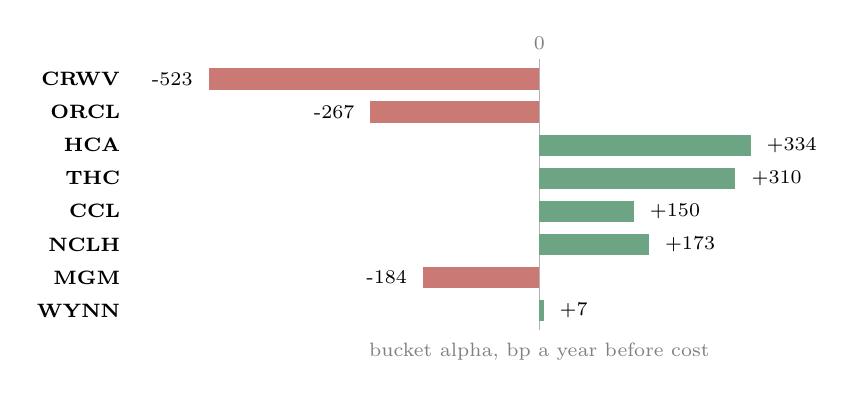
\begin{tikzpicture}[x=1cm,y=0.42cm,font=\scriptsize]
\draw[gray!60] (0,0.6) -- (0,-7.6);
\node[gray,anchor=south] at (0,0.6) {0};
\node[anchor=east] at (-5.20,0) {\textbf{CRWV}};
\fill[bad!70] (0,-0.32) rectangle (-4.200,0.32);
\node[anchor=east] at (-4.280,0) {-523};
\node[anchor=east] at (-5.20,-1) {\textbf{ORCL}};
\fill[bad!70] (0,-1.32) rectangle (-2.145,-0.68);
\node[anchor=east] at (-2.225,-1) {-267};
\node[anchor=east] at (-5.20,-2) {\textbf{HCA}};
\fill[good!70] (0,-2.32) rectangle (2.683,-1.68);
\node[anchor=west] at (2.763,-2) {+334};
\node[anchor=east] at (-5.20,-3) {\textbf{THC}};
\fill[good!70] (0,-3.32) rectangle (2.491,-2.68);
\node[anchor=west] at (2.571,-3) {+310};
\node[anchor=east] at (-5.20,-4) {\textbf{CCL}};
\fill[good!70] (0,-4.32) rectangle (1.201,-3.68);
\node[anchor=west] at (1.281,-4) {+150};
\node[anchor=east] at (-5.20,-5) {\textbf{NCLH}};
\fill[good!70] (0,-5.32) rectangle (1.392,-4.68);
\node[anchor=west] at (1.472,-5) {+173};
\node[anchor=east] at (-5.20,-6) {\textbf{MGM}};
\fill[bad!70] (0,-6.32) rectangle (-1.476,-5.68);
\node[anchor=east] at (-1.556,-6) {-184};
\node[anchor=east] at (-5.20,-7) {\textbf{WYNN}};
\fill[good!70] (0,-7.32) rectangle (0.054,-6.68);
\node[anchor=west] at (0.134,-7) {+7};
\node[anchor=north,gray] at (0,-7.7) {bucket alpha, bp a year before cost};
\end{tikzpicture}
}\\[3pt]
{\scriptsize\textbf{Rest of G2 (E0, E1, E2, E3, E6), 18\%}}\\[1pt]
\scalebox{0.8}{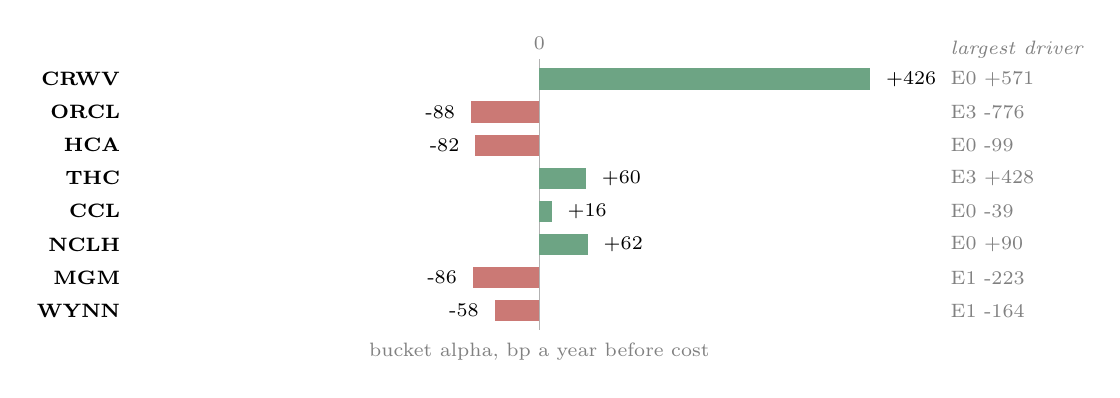
\begin{tikzpicture}[x=1cm,y=0.42cm,font=\scriptsize]
\draw[gray!60] (0,0.6) -- (0,-7.6);
\node[gray,anchor=south] at (0,0.6) {0};
\node[anchor=east] at (-5.20,0) {\textbf{CRWV}};
\fill[good!70] (0,-0.32) rectangle (4.200,0.32);
\node[anchor=west] at (4.280,0) {+426};
\node[anchor=west,gray] at (5.10,0) {E0 +571};
\node[anchor=east] at (-5.20,-1) {\textbf{ORCL}};
\fill[bad!70] (0,-1.32) rectangle (-0.868,-0.68);
\node[anchor=east] at (-0.948,-1) {-88};
\node[anchor=west,gray] at (5.10,-1) {E3 -776};
\node[anchor=east] at (-5.20,-2) {\textbf{HCA}};
\fill[bad!70] (0,-2.32) rectangle (-0.812,-1.68);
\node[anchor=east] at (-0.892,-2) {-82};
\node[anchor=west,gray] at (5.10,-2) {E0 -99};
\node[anchor=east] at (-5.20,-3) {\textbf{THC}};
\fill[good!70] (0,-3.32) rectangle (0.590,-2.68);
\node[anchor=west] at (0.670,-3) {+60};
\node[anchor=west,gray] at (5.10,-3) {E3 +428};
\node[anchor=east] at (-5.20,-4) {\textbf{CCL}};
\fill[good!70] (0,-4.32) rectangle (0.156,-3.68);
\node[anchor=west] at (0.236,-4) {+16};
\node[anchor=west,gray] at (5.10,-4) {E0 -39};
\node[anchor=east] at (-5.20,-5) {\textbf{NCLH}};
\fill[good!70] (0,-5.32) rectangle (0.614,-4.68);
\node[anchor=west] at (0.694,-5) {+62};
\node[anchor=west,gray] at (5.10,-5) {E0 +90};
\node[anchor=east] at (-5.20,-6) {\textbf{MGM}};
\fill[bad!70] (0,-6.32) rectangle (-0.844,-5.68);
\node[anchor=east] at (-0.924,-6) {-86};
\node[anchor=west,gray] at (5.10,-6) {E1 -223};
\node[anchor=east] at (-5.20,-7) {\textbf{WYNN}};
\fill[bad!70] (0,-7.32) rectangle (-0.567,-6.68);
\node[anchor=east] at (-0.647,-7) {-58};
\node[anchor=west,gray] at (5.10,-7) {E1 -164};
\node[anchor=north,gray] at (0,-7.7) {bucket alpha, bp a year before cost};
\node[anchor=west,gray,font=\scriptsize\itshape] at (5.10,0.9) {largest driver};
\end{tikzpicture}
}
\end{center}
\begin{itemize}
\item The clocks score CRWV, ORCL and MGM as negative. They score the hospitals and the cruise lines as positive.
\item In the rest of G2, CRWV is highest ($+648$). Its spread level ($+571$) and its pair gap ($+1{,}950$) drive it.
\item E3 gives the two legs of a pair the same size with opposite signs. So CRWV gets $+1{,}950$ and ORCL gets $-1{,}950$. Against the peer fair spread the pair gap is 400 bp, not 159 bp. These sizes are not calibrated.
\end{itemize}

\fld{Evidence and limits}
\begin{itemize}
\item The alpha backtest (2008 to 2026) supports spread level and the old leverage line. Their rank IC after cost is 0.22 to 0.29 with the $\beta = 1$ hedge. The peer fair spread that replaced the line adds beyond spread level in 3 of 4 cycles at 3 and 12 months. Its sizes do not calibrate.
\item The size is too large: realised alpha is about 0.08 times the predicted alpha. S14b applies that slope.
\item The clocks backtest (2018 to 2026, 1,143 issuers) does not support E5. Its IC after cost is $-0.08$ to $-0.11$. Beyond the spread rank it is not different from zero.
\item The market already prices the clocks. Issuers with heavy fixed charges pay more spread.
\item E1, E2 and E10 all use the peer fair spread, and E14 measures the same gap. So the peer gap counts more than any one weight shows.
\end{itemize}

\fld{The test that settles its weight}
The clocks test is done and does not support the 20\%. The user keeps the 20\% by choice. For the rest, set each weight in proportion to its rank IC after cost in each cycle phase. Keep the combination only if it beats ``buy the widest'' after cost in three of the four cycles.

% ---------------------------------------------------------------------------------------------------------------
\newpage
\section*{\textcolor{gC}{G3} Credit skills}
\addcontentsline{toc}{section}{G3 Credit skills}

\begin{notebox}
\textbf{In one line.} G3 adds the checklists of seven credit skills. It can only lower the number. It carries 5\%.
\end{notebox}

\fld{What it is}
G3 is seven skill files. One is written for this project. Six are written for private loans and adapted here to public bonds:
\begin{itemize}
\item \code{hy-model-standards} (this project) and \code{credit-model-standards}: debt at face, three EBITDAs, the FCF cross-check, a severe case from the issuer's own main risk.
\item \code{ebitda-addback-treatment}: the bridge from reported to adjusted EBITDA, with limits on each add-back.
\item \code{covenant-compliance}: headroom bands and the direction of headroom over time.
\item \code{borrower-monitoring}: trend per line and the watchlist tiers.
\item \code{credit-memo-standards} and \code{quarterly-package-extraction}: what a memo must hold, and how to read a statement package.
\end{itemize}
Code: \code{hy/skills.py}.

\fld{Why it is in the framework}
G3 holds the checks that an experienced lender runs every quarter. They catch problems that the price models do not see. A clean checklist earns no credit, because a clean result is the normal case. So G3 is one-way.

\fld{What does not transfer to public bonds}
The code lists six rules that do not transfer (\code{NOT_TRANSFERABLE}):
\begin{enumerate}
\item No compliance certificate exists for public bonds. The code computes its own ratio against a level parsed from the filing text.
\item Equity cures and step-downs need the credit agreement and monthly revolver data.
\item No sponsor plan is public. The proxy is the same quarters a year earlier.
\item Add-back caps live in the credit agreement. Compustat gives one special-items line.
\item Sources and uses at entry apply to new loans, not to bonds bought in the market.
\end{enumerate}
The sixth rule: monthly lender packages do not exist. XBRL quarters replace them.

\fld{What it adds at each step}
{\footnotesize
\begin{tabularx}{\linewidth}{@{}>{\raggedright\arraybackslash}p{24mm}>{\raggedright\arraybackslash}X@{}}
\toprule
Step & G3 contribution \\
\midrule
S1 Load & Bridge the debt between the balance sheet and the documents. Flag a new line item. Do not guess its place. \\
S2 Business & A top customer above 15 to 20\% of revenue makes the loss of that customer the downside. \\
S3 Earnings & Flag one add-back above 5\% of EBITDA, a total above 10\%, or the same add-back for three quarters. FCF cross-check within 15\%. \\
S4 Liquidity & Thin liquidity or a maturity with no refinance path puts a name on the watchlist, even when EBITDA holds. \\
S5 Claims & Debt at face. Headroom bands: comfortable above 20\%, tight below 10\%. Flag a falling path early. \\
S7 Cases & The severe case combines a revenue fall, a margin squeeze and working-capital stress. Report the first breach quarter. \\
S8 Value & Loan to value moves with the sector multiple, even when leverage does not. \\
S11 Gate & A memo without its key risk fails. A ``pass'' is a normal outcome. \\
S12 Events & Watchlist tiers from the trend: watch closely at 10\% below the prior year, watchlist at 20\%. \\
\bottomrule
\end{tabularx}
}
No skill covers relative value (S9) or expected return (S10). The skills judge debt service, not price.

\newpage
\fld{Its estimate in the score}
{\footnotesize
\begin{tabularx}{\linewidth}{@{}>{\raggedright\arraybackslash}p{8mm}>{\raggedright\arraybackslash}p{34mm}>{\raggedright\arraybackslash}X>{\raggedright\arraybackslash}p{12mm}@{}}
\toprule
ID & Estimate & How the code computes it & Weight \\
\midrule
E11 & Watchlist and covenant path & Minus the watchlist tier (0 none, 1 watch closely, 2 watchlist, 3 workout), minus one if headroom falls. Standardised, then capped at zero. & 5\% \\
\bottomrule
\end{tabularx}
}
E7 (earnings quality) also comes from the skills and is also one-way. The code counts it in G1.

\fld{What it says about the eight issuers}
\begin{center}
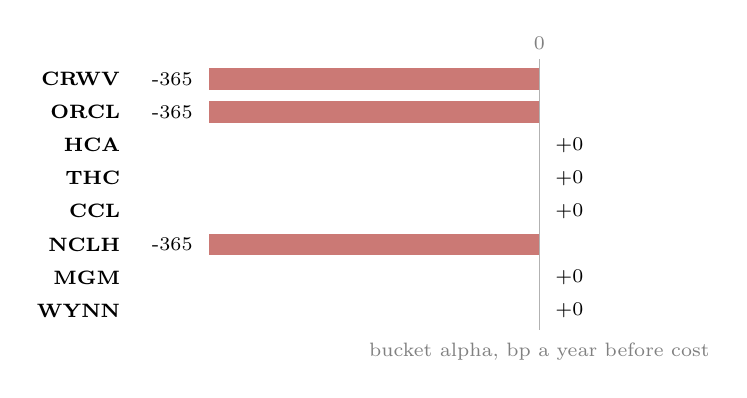
\begin{tikzpicture}[x=1cm,y=0.42cm,font=\scriptsize]
\draw[gray!60] (0,0.6) -- (0,-7.6);
\node[gray,anchor=south] at (0,0.6) {0};
\node[anchor=east] at (-5.20,0) {\textbf{CRWV}};
\fill[bad!70] (0,-0.32) rectangle (-4.200,0.32);
\node[anchor=east] at (-4.280,0) {-365};
\node[anchor=east] at (-5.20,-1) {\textbf{ORCL}};
\fill[bad!70] (0,-1.32) rectangle (-4.200,-0.68);
\node[anchor=east] at (-4.280,-1) {-365};
\node[anchor=east] at (-5.20,-2) {\textbf{HCA}};
\node[anchor=west] at (0.080,-2) {+0};
\node[anchor=east] at (-5.20,-3) {\textbf{THC}};
\node[anchor=west] at (0.080,-3) {+0};
\node[anchor=east] at (-5.20,-4) {\textbf{CCL}};
\node[anchor=west] at (0.080,-4) {+0};
\node[anchor=east] at (-5.20,-5) {\textbf{NCLH}};
\fill[bad!70] (0,-5.32) rectangle (-4.200,-4.68);
\node[anchor=east] at (-4.280,-5) {-365};
\node[anchor=east] at (-5.20,-6) {\textbf{MGM}};
\node[anchor=west] at (0.080,-6) {+0};
\node[anchor=east] at (-5.20,-7) {\textbf{WYNN}};
\node[anchor=west] at (0.080,-7) {+0};
\node[anchor=north,gray] at (0,-7.7) {bucket alpha, bp a year before cost};
\end{tikzpicture}

\end{center}
\begin{itemize}
\item Three issuers are on the watchlist: CRWV, ORCL and NCLH. Each gets $-365$ bp a year.
\item The other five have no tier. They get zero, not a credit.
\item So G3 can only pull the combined number down. For CRWV it removes 18 bp a year after its 5\% weight.
\item Covenant headroom is ``open'' for seven of the eight issuers. The code parsed no covenant level from their filings. So the headroom term rarely fires.
\end{itemize}

\fld{Evidence and limits}
\begin{itemize}
\item No backtest covers E11 yet.
\item The thresholds come from the skills. The skills set them for private loans, not for public bonds.
\item The plan proxy (the same quarters a year earlier) is weaker than a real plan. A fast grower can look safe when its plan was higher.
\item Three of eight issuers share one value. So the bucket separates names in two groups only.
\end{itemize}

\fld{The test that settles its weight}
Build the watchlist tier point in time for the backtest panel. Test whether a tier above zero predicts a lower hedged return over six months, beyond the spread rank. If it does not, keep G3 in the memo as a risk flag and remove its weight.

% ---------------------------------------------------------------------------------------------------------------
\newpage
\section*{\textcolor{gD}{G4} Books and peers}
\addcontentsline{toc}{section}{G4 Books and peers}

\begin{notebox}
\textbf{In one line.} G4 adds two textbook cross-checks and three peer signals that use no repository model. It carries 17\%.
\end{notebox}

\fld{What it is}
G4 is three books:
\begin{itemize}
\item Kricheff, \emph{A Pragmatist's Guide to Leveraged Finance} (2nd edition). It is a practitioner's view of high yield: cash flow, spread per turn of leverage, covenants, events.
\item Ganguin and Bilardello, \emph{Standard \& Poor's Fundamentals of Corporate Credit Analysis} (2005). It is the S\&P rating method: business risk, adjusted ratios, medians by rating, recovery.
\item Dynkin et al., \emph{Systematic Investing in Credit} (2021), ch.~13 and 14. It is the Barclays research on value and momentum in credit: ESP, SPiDER and OneScore.
\end{itemize}
Code: \code{hy/books.py} and \code{hy/peers.py}. The text comes from markdown conversions of the three books. No other book is in scope, and Fabozzi is excluded.

\fld{Why it is in the framework}
G4 checks the price with methods that do not depend on our models. If our model and a textbook method agree, the call is stronger. If they disagree, the memo must explain why.

\fld{What it adds at each step}
{\footnotesize
\begin{tabularx}{\linewidth}{@{}>{\raggedright\arraybackslash}p{24mm}>{\raggedright\arraybackslash}X@{}}
\toprule
Step & G4 contribution \\
\midrule
S1 Load & Start from the filed statements and the bond terms. Use several years of history. \\
S2 Business & S\&P: industry risk sets a ceiling on the issuer's grade. \\
S3 Earnings & Kricheff: reconcile every EBITDA and FCF figure to cash from operations. The analyst may reject new-issue add-backs. \\
S4 Liquidity & Kricheff: restricted cash does not count. A revolver counts only if the issuer can draw it. Never assume a refinance. \\
S5 Claims & Kricheff: leverage at each tranche level, structural subordination. S\&P: add leases and pensions to debt. \\
S6 Clocks & S\&P: forecast past the maturity when refinance risk exists. Kricheff: PIK debt raises the claim without cash. \\
S7 Cases & S\&P: stress the worst credible case. A high-risk issuer takes a 10 to 30\% revenue fall at the start. \\
S8 Value & S\&P: name the default type, value at emergence, discount the recovery for time at 10\%. \\
S9 Relative value & Kricheff: use spread to worst. A junior note must pay more per turn than a senior note. \\
S10 Alpha & Kricheff: yield to worst is the base return. S\&P: expected loss is PD times LGD times exposure. \\
S11 Gate & S\&P: decide on the three to five issues that matter. Soft factors can only lower a grade. \\
S12 Events & Kricheff: pro formas for an acquisition, a takeover, an IPO, a call. \\
S13 Metrics & S\&P ratio medians by rating. Kricheff's ratios: (EBITDA $-$ capex) over interest, FCF over debt. \\
S15 Decision & Kricheff: define the mandate first. Ask whether a better instrument exists. \\
\bottomrule
\end{tabularx}
}

\newpage
\fld{Its estimates in the score}
{\footnotesize
\begin{tabularx}{\linewidth}{@{}>{\raggedright\arraybackslash}p{8mm}>{\raggedright\arraybackslash}p{34mm}>{\raggedright\arraybackslash}X>{\raggedright\arraybackslash}p{12mm}@{}}
\toprule
ID & Estimate & How the code computes it & Weight \\
\midrule
E12 & Ratio-implied rating gap & $z(\log s) - z(\text{S\&P score})$. The S\&P score (1 best, 10 worst) blends a business score and a financial score from the 2002 medians. A wide spread for the score is cheap. & 2.5\% \\
E13 & Spread per turn against peers & $\log(\text{spread}/\text{leverage})$ minus the median of peers in the same GICS sector, rating class and maturity bucket. It is zero on Kricheff's trap guard: FCF over debt at or below zero, value cover at or below 1, or two of high leverage, low FCF over debt and a thin cushion. & 2.5\% \\
E14 & Excess spread to peers (ESP) & $\log(\text{spread})$ minus the median of peers in the same GICS sector, rating class and maturity bucket. Dynkin et al.\ ch.~13, without their leverage control: the control halved the edge in our backtest. & 4.5\% \\
E15 & SPiDER & $\log\big(\text{spread} / (\text{debt} / \text{10-year mean EBITDA})\big)$, one rank across all sectors. None for a financial issuer or with fewer than 6 annual EBITDA figures. Dynkin et al.\ ch.~14. & 3\% \\
E16 & OneScore & Mean of the within-sector ranks of issuer ESP and the 3-month stock return. An unlisted issuer takes its ESP value. Dynkin et al.\ ch.~19. & 4.5\% \\
\bottomrule
\end{tabularx}
}

\fld{What it says about the eight issuers}
\begin{center}
\scalebox{0.72}{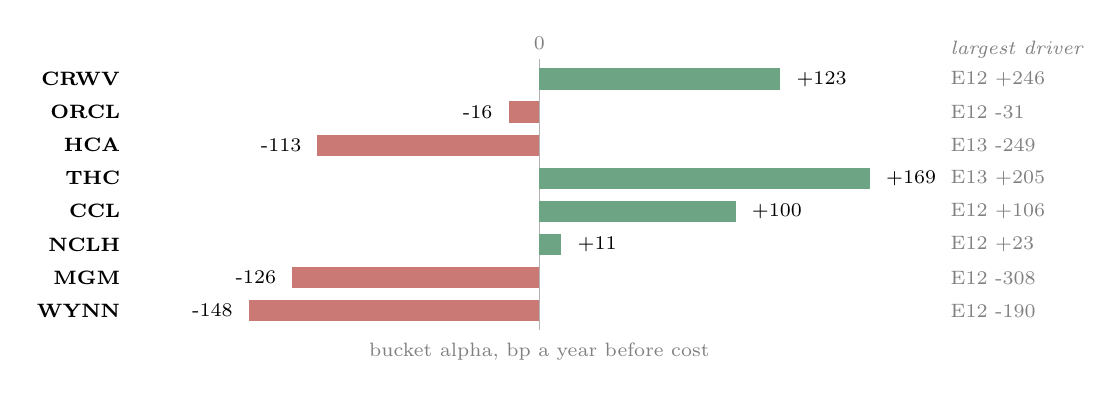
\begin{tikzpicture}[x=1cm,y=0.42cm,font=\scriptsize]
\draw[gray!60] (0,0.6) -- (0,-7.6);
\node[gray,anchor=south] at (0,0.6) {0};
\node[anchor=east] at (-5.20,0) {\textbf{CRWV}};
\fill[good!70] (0,-0.32) rectangle (3.062,0.32);
\node[anchor=west] at (3.142,0) {+123};
\node[anchor=west,gray] at (5.10,0) {E12 +246};
\node[anchor=east] at (-5.20,-1) {\textbf{ORCL}};
\fill[bad!70] (0,-1.32) rectangle (-0.391,-0.68);
\node[anchor=east] at (-0.471,-1) {-16};
\node[anchor=west,gray] at (5.10,-1) {E12 -31};
\node[anchor=east] at (-5.20,-2) {\textbf{HCA}};
\fill[bad!70] (0,-2.32) rectangle (-2.818,-1.68);
\node[anchor=east] at (-2.898,-2) {-113};
\node[anchor=west,gray] at (5.10,-2) {E13 -249};
\node[anchor=east] at (-5.20,-3) {\textbf{THC}};
\fill[good!70] (0,-3.32) rectangle (4.200,-2.68);
\node[anchor=west] at (4.280,-3) {+169};
\node[anchor=west,gray] at (5.10,-3) {E13 +205};
\node[anchor=east] at (-5.20,-4) {\textbf{CCL}};
\fill[good!70] (0,-4.32) rectangle (2.496,-3.68);
\node[anchor=west] at (2.576,-4) {+100};
\node[anchor=west,gray] at (5.10,-4) {E12 +106};
\node[anchor=east] at (-5.20,-5) {\textbf{NCLH}};
\fill[good!70] (0,-5.32) rectangle (0.281,-4.68);
\node[anchor=west] at (0.361,-5) {+11};
\node[anchor=west,gray] at (5.10,-5) {E12 +23};
\node[anchor=east] at (-5.20,-6) {\textbf{MGM}};
\fill[bad!70] (0,-6.32) rectangle (-3.139,-5.68);
\node[anchor=east] at (-3.219,-6) {-126};
\node[anchor=west,gray] at (5.10,-6) {E12 -308};
\node[anchor=east] at (-5.20,-7) {\textbf{WYNN}};
\fill[bad!70] (0,-7.32) rectangle (-3.691,-6.68);
\node[anchor=east] at (-3.771,-7) {-148};
\node[anchor=west,gray] at (5.10,-7) {E12 -190};
\node[anchor=north,gray] at (0,-7.7) {bucket alpha, bp a year before cost};
\node[anchor=west,gray,font=\scriptsize\itshape] at (5.10,0.9) {largest driver};
\end{tikzpicture}
}
\end{center}
\begin{itemize}
\item CRWV is highest ($+353$). It pays 78\% more than its peers (E14 $+527$), and its spread is wide for its S\&P score (E12 $+417$). It has no E13 (it burns cash, so the trap guard sets it to zero) and no SPiDER (3 years of EBITDA).
\item HCA is lowest ($-262$): it pays 52\% less than its peers (E14 $-476$). THC rises to $+313$ because its stock is up 52\% in 3 months (E16 $+508$).
\item For MGM the books say tight (E12 $-523$), and SPiDER now agrees ($-417$). SPiDER was $+363$ on 22 October. The change comes from the debt figure. The peer cells now use the panel's point-in-time debt for every issuer: \$31.7bn for MGM, against \$6.1bn in step 5. What makes up the gap is an open question.
\end{itemize}

\fld{Evidence and limits}
\begin{itemize}
\item The peer backtest (2008 to 2026) finds that E13 adds nothing beyond spread level: IC beyond spread $+0.02$, $t$ 1.1. No backtest covers E12 yet.
\item ESP adds information beyond spread level: $+0.07$ at 6 months and $+0.10$ at 12 months ($t$ 2.6). But the edge disappears in the 2008 and 2020 stress windows. OneScore adds stock momentum and passes three of four cycles beyond spread (+0.034, $t$ 2.1). ESP and OneScore share 9\%. Decision pages: \code{2026-10-22-esp-peer-groups} and \code{2026-10-22-weights-esp-spider}.
\item SPiDER adds $+0.03$ beyond spread at 12 months ($t$ 1.3), and $+0.06$ ($t$ 1.6) on the book's February schedule. Its 3\% reflects that weak support.
\item No rating source covers 2017 onward. After 2017, the rating class comes from leverage. It matches the actual class on 36\% of issuer-months.
\item The S\&P medians date from 2002. The Kricheff conversion lost every table, so only numbers quoted in the text survive.
\end{itemize}

\fld{The test that settles its weight}
Compute the S\&P score and the spread per turn point in time on the backtest panel. Test each one's rank IC after cost beyond the spread rank. E12 is close to the fair line in idea. If it adds nothing beyond E2, drop it. Rerun ESP and SPiDER with OAS and a rating feed after 2017. Keep the 9\% for ESP and OneScore if they pass the cycle bar. Move E13's weight to SPiDER if SPiDER passes $t$ 2.


\newpage
\tableofcontents
\newpage
%======================================================================
\section{S1 Load the data}\label{s1}

\textbf{Purpose.} Load every input with the date the market could first read it, so that no later step sees the future.

\fld{What each group contributes}
\begin{itemize}
\item \GA{} The rule: every field carries \code{as_of} and \code{available_at}; a memo dated $t$ reads nothing released after $t$ (M3, F1 R5). Every number cites its source line (R4). The PDF adds: list the feasible opportunity set first (R7--R9); TRACE prices are estimates, not executable quotes (R10); verify clean, dirty or flat per bond (R16); dirty price and market value (U1, U2).
\item \GB{} The live loaders: Compustat point-in-time quarters, XBRL instances with dimensions, EDGAR acceptance times, TRACE (10-day volume-weighted yields), Treasury par curves, and the forecast registry with five live sources (SPF, FOMC SEP, Treasury forwards, SLOOS, TRACE HY level).
\item \GC{} \code{quarterly-package-extraction}: read the statements top down; aggregate months to quarters to LTM; flag any new line item instead of guessing its place. The debt must always bridge between balance sheet and document (OID, leases, letters of credit). In public HY there is no compliance certificate; the 10-Q and the indenture replace it.
\item \GD{} Both books start from the filed statements and the bond terms. S\&P adds that the analyst should use several years of history and adjust the statements before any ratio (see S3).
\end{itemize}

\fld{Algorithm}
\begin{algobox}
\begin{enumerate}
\item Set the decision time $t$ = last TRACE date + 1 day.
\item For each issuer, read the latest 10-Q or 10-K with acceptance time $\le t$. Parse the XBRL instance with dimensions.
\item Read Compustat point-in-time quarters known at $t$. Fill a missing fourth quarter from XBRL as first filed (decision page \code{2026-10-21-pit-financials-sources}). Rebuild quarterly flows from year-to-date by differences.
\item Read TRACE bonds: fixed coupon, not convertible, senior unsecured or secured, 1 to 15 years, price $\ge$ 80. Compute G-spreads on the curve of $t$.
\item Read every forecast row with \code{available_at} $\le t$; keep the newest vintage per source and variable.
\item Reconcile debt: balance-sheet debt against the maturity ladder; put an unexplained gap in the tail and log it.
\item Write each value with its source line and \code{available_at}. A value without a source is an open question.
\end{enumerate}
\end{algobox}

\fld{Metrics}
\begin{equation}
s^{G}_b = y_b - y^{UST}(T_b),\qquad P^{d}_b = P^{c}_b + AI_b,\qquad X^{LTM}_t = \sum_{q=t-3}^{t} X_q .
\end{equation}
\intu{the G-spread is the bond's pay over a Treasury of the same maturity; the dirty price is what a buyer pays; LTM adds the last four quarters.}
\sym{$y_b$ volume-weighted TRACE yield of bond $b$; $y^{UST}(T)$ Treasury par yield at maturity $T_b$ (years); $P^c$ clean price; $AI$ accrued interest; $X_q$ a quarterly flow.}

\fld{Bands} None. Data quality flags: debt ladder does not reconcile within 5\%; a quarter missing; a bond with no trade in 10 days.

\fld{Inputs} \emph{Data:} Compustat, XBRL, EDGAR, TRACE, Treasury, forecast registry. \emph{Documents:} 10-K and 10-Q text. \emph{Analyst:} ticker list, pairs, overrides in \code{data/analyst_inputs/<ticker>.yaml}.

\fld{Outputs} \code{filing}, \code{bonds_priced}, \code{curve_basis}, \code{decision_time}, and the source of every LTM figure.

\fld{Where groups disagree} G1 (M3.1) says US bonds quote clean; the PDF (R16) says verify per bond (C18). \textbf{Wins:} a per-bond \code{quote_convention} field with M3.1 as default, because bonds near default trade flat. G3 treats the certificate as the source of truth (K6); public HY has none, so the filing and the indenture win.

\fld{Settling test} Code tests: \code{tests/test_inputs.py}; \code{tests/test_forecasts.py::test_as_of_never_reads_rows_released_later}, \code{tests/test_sources.py}, \code{tests/test_xbrl.py}, \code{tests/test_trace_bonds.py::test_g_spread_arithmetic_and_no_look_ahead}. Open: the M11 point-in-time replay of every feature.

\fld{Status} \stpartial. Missing: ratings, face and call schedule by bond, accrued interest, quote convention, bid and ask, consensus, guidance, default labels, ICE OAS.
%======================================================================
\section{S2 Frame the business}\label{s2}

\textbf{Purpose.} Decide what kind of business this is and how risky it is before any debt, because that sets which earnings, ratios, downside and events matter.

\fld{What each group contributes}
\begin{itemize}
\item \GA{} Gatto step 2 (Chapter 6, pp.~155--186): eight industry risks (Figure 6.2, p.~158), the strategy, management, ESG. F2: five lines (what it sells, how one unit earns, what it must spend to stand still, market structure, what breaks it); one archetype A1--A8; modifiers M1 sponsor, M2 secular decline, M3 concentration. M4.4: each risk scored 0, 1 or 2. PDF: three to five material risks, each tied to a downside case (P4); an evidence ledger (P5); risk must change the forecast, not be added to a ratio (R31, R34); undisclosed concentration is missing, not zero (R32).
\item \GB{} The code reads the archetype from the analyst file, the first two sentences of 10-K Item 1, the XBRL customer shares, and the F2 downside driver of the archetype.
\item \GC{} \code{credit-model-standards}: the downside comes from the business's own risk profile, never from another deal's template; a top customer above 15--20\% of revenue makes loss of that customer the downside. \code{credit-memo-standards}: state the business in one sentence first.
\item \GD{} S\&P (Ganguin and Bilardello, Ch.~1--4, 10): grade country, industry and company risk; industry risk sets a ceiling on the issuer (Table 2-2 ranks steel, autos, airlines, homebuilders and paper highest; branded consumer, pharma and regulated utilities lowest); find the sector's keys to success and the driver under each; score each key 1--10 and weight them into a business risk score (forest products: cost 50\% $\times$ 7, diversity 30\% $\times$ 8, integration 20\% $\times$ 4 gives 6.7); management's past deviation from plan predicts future deviation; seventeen governance red flags. Kricheff (Ch.~11, 19, 25): competition, concentration, barriers, cyclicality, capital intensity, price setter or taker; private-equity owners almost ensure a transaction; test management targets against peers (a 15\% margin target where no peer exceeds 12\% deserves doubt).
\end{itemize}

\fld{Algorithm}
\begin{algobox}
\begin{enumerate}
\item Write the five F2 lines. Cite the 10-K for each.
\item Assign one archetype. If two fit, compute both views later and report the difference (F2.1).
\item Set modifiers: M1 if a sponsor owns it; M2 if industry volume falls over five years with no cyclical cause; M3 if the top customer is above 20\% of revenue. Raise a watch flag at 15\%.
\item Score the business risk profile on the G4 scale (country, industry, competitive position) from the evidence in step 1: weight the sector keys to success, score each 1--10, and cap the result at the industry ceiling (S\&P). Governance red flags can only make the score worse, never better.
\item Name three to five material risks. For each, name the forecast driver it changes and the downside case that carries it (to S7). Do not add the scores to any ratio.
\item Re-frame on a change of business mix above 20\% of revenue, an acquisition, or a change of owner (F2.4).
\end{enumerate}
\end{algobox}

\fld{Metrics}
\begin{equation}
HHI = \sum_j \Big(\frac{Rev_j}{Rev}\Big)^2,\qquad top_1 = \max_j \frac{Rev_j}{Rev}.
\end{equation}
\intu{revenue held by few customers can vanish in one step.}
\sym{$Rev_j$ revenue from customer $j$ (XBRL concentration axis); undisclosed shares stay missing.}
\begin{equation}
BR = \sum_k \omega_k\, b_k,\qquad \sum_k \omega_k = 1,\qquad BR \ge BR^{ind}.
\end{equation}
\intu{the business risk score is a weighted grade of what wins in this industry, never better than the industry allows.}
\sym{$b_k\in[1,10]$ score on key to success $k$ (1 best); $\omega_k$ its weight; $BR^{ind}$ the best score the industry allows (S\&P industry ranking).}

\fld{Bands} $top_1$: below 15\% green; 15--20\% amber (watch); above 20\% red (M3). Business risk score $BR$: 1--4 low, 5--6 moderate, 7--10 high (S\&P scale; cut points v0).

\fld{Inputs} \emph{Data:} customer shares, LTM revenue, EBITDA, lease cost. \emph{Documents:} 10-K Item 1 and risk factors. \emph{Analyst:} archetype, modifiers M1 and M2, market structure, the business risk grade.

\fld{Outputs} \code{archetype}, \code{modifiers}, \code{sells}, \code{earns}, \code{breaks}, \code{market_structure}, \code{business_risk}, \code{material_risks[]}.

\fld{Where groups disagree} G3 sets concentration at 15--20\%; F2 at 20\% (K7). \textbf{Wins:} 20\% for the modifier and 15\% for a watch flag, because the modifier changes the case set and needs a firmer trigger. G1 M4.4 feeds scores into the fair model; the PDF forbids adding scores to ratios (C16). \textbf{Wins:} the scenario route; a score vector enters a model only after the R163 admission test. G4 (S\&P) combines business and financial scores into one grade (B4). \textbf{Wins:} keep the S\&P grade only as a cross-check estimate in S14, never as a term in a spread or PD model.

\fld{Settling test} F13 blind memo rubric, item 1, on held-out resolved credits. For the score: ablate it from the fair model; keep it only if out-of-sample residual variance falls.

\fld{Status} \stpartial. Built: archetype, M3, ``sells'' and ``breaks''. Missing: market structure, M1, M2, material risks, the business risk grade, re-frame triggers.

\fld{CRWV} Archetype A5 (asset-heavy contracted); M3, the largest customer is 36\% of revenue; revenue 7.6bn a year at a 50\% EBITDA margin; rent 2.07bn a year.
%======================================================================
\section{S3 Normalise earnings and add-backs}\label{s3}

\textbf{Purpose.} Find the earnings and the cash that recur, and flag accounts that look better than the cash.

\fld{What each group contributes}
\begin{itemize}
\item \GA{} Gatto step 3a (Chapter 7, pp.~187--223): remove nonrecurring items (Figure 7.3, p.~192); a ``nonrecurring'' charge that recurs is an operating cost. F3: three EBITDA numbers kept apart (analyst, company, covenant); add-back classes C1--C10 (C6 stock compensation never; C8 projected synergies never); history of 3--5 years, a full cycle for A3 and A4; quality tests EQ1--EQ10. M4.2: FCF from adjusted EBITDA less the cash part of the add-backs. PDF: a repeated cash cost is not nonrecurring (R37); Gatto's five quality tests (P9); backlog bridge and book-to-bill (E16, E17); add-back dependence (E71); cash conversion (E72); no double count from a CFO start (R42).
\item \GB{} The code runs EQ1, EQ2, EQ5, EQ7, the 8-quarter margin trend, and FCF as CFO less capex.
\item \GC{} \code{ebitda-addback-treatment}: build net income to reported EBITDA first, then layer each covenant add-back; split cash from non-cash add-backs; flag a category above 5\% of EBITDA, the same add-back for 3--4 quarters, and small items that sum above 10--15\%; track whether add-backs roll off. \code{hy-model-standards}: a synergy enters FCF only from the quarter it shows in reported EBITDA; cross-check FCF against CFO less capex. \code{quarterly-package-extraction}: an acquisition folded into reported numbers inflates growth; separate organic from acquired.
\item \GD{} Kricheff (Ch.~9, 10, 16, 22): build EBITDA as net income + tax + interest + D\&A; reconcile every EBITDA and FCF figure to cash from operations; footnote each add-back; the analyst may reject new-issue add-backs (sponsor fees, full planned savings, restructuring cash); normalise capex (a 75m one-off data centre inside 200m of capex leaves 125m recurring); show analyst and covenant EBITDA side by side; capex that stays below depreciation predicts a capex spike. S\&P (Ch.~5, 6): spread 3--5 years; run the accounting checklist (auditor changes, restatements, consolidation, LIFO, pensions, securitisation, capitalised costs, net income that grows faster than cash flow); define FFO, OCF, FOCF and discretionary cash flow; compute hybrids at 0\% and at 100\% debt.
\end{itemize}

\fld{Algorithm}
\begin{algobox}
\begin{enumerate}
\item Build reported EBITDA from the statements: net income + tax + interest + D\&A. Tie it to the issuer's own EBITDA. If it does not tie, log the gap.
\item List every item between reported and company-adjusted EBITDA (8-K exhibit 99). Classify each as C1--C10 (F3). Mark it cash or non-cash.
\item Decide each item by the F3 rule. Reject: stock compensation (C6), projected synergies (C8), any item present in 3 of the last 5 years (C2, EQ5), or 3--4 quarters in a row at a similar level (G3).
\item Analyst EBITDA $E^{adj}$ = reported + accepted items. Company EBITDA as reported. Covenant EBITDA by the indenture definition (or the 10-Q covenant note).
\item Compute FCF by the M4.2 identity. Compute the cross-check $CFO - Capex$. Flag a gap above 15\% of $E^{adj}$.
\item Run EQ1--EQ10. Count the flags; EQ10 counts twice.
\item Compute the margin trend over 8 quarters and the organic growth (Gatto definition, C17).
\item Compute the S\&P cash ladder (FFO, OCF, FOCF, discretionary cash flow). Run the S\&P accounting checklist; each failed item counts as an EQ10-type flag.
\end{enumerate}
\end{algobox}

\fld{Metrics}
\begin{equation}
E^{adj}_t = E^{rep}_t + \sum_i a_i\,NR_{i,t},\qquad FCF_t = E^{adj}_t - CashNR_t - K_t - I^{c}_t - T^{c}_t - \Delta WC_t .
\end{equation}
\intu{add back only what will not recur, then charge the cash that the add-backs hid.}
\sym{$NR_{i,t}$ nonrecurring item $i$; $a_i\in\{0,1\}$ the add-back decision; $CashNR_t$ cash part of accepted items; $K$ capex; $I^c$ cash interest; $T^c$ cash tax; $\Delta WC$ working-capital build.}
\begin{equation}
gap^{add} = \frac{E^{co}}{E^{adj}} - 1,\qquad gap^{cov} = \frac{E^{cov}}{E^{adj}} - 1,\qquad chk = \frac{FCF - (CFO - K)}{E^{adj}} .
\end{equation}
\intu{how far the issuer's and the document's earnings sit above the analyst's, and how far the model's FCF sits from the cash flow statement.}
\sym{$E^{co}$ company-adjusted EBITDA; $E^{cov}$ covenant EBITDA; $CFO$ operating cash flow.}
\begin{equation}
conv = \frac{\sum_{4q}(CFO - K)}{\sum_{4q} E},\qquad trend = \frac{\hat b}{\mathrm{se}(\hat b)},\qquad
\text{EQ1} = 1\Big\{\frac{DSO_t}{DSO_{t-4}} - 1 > 0.10 \wedge g < 0.05\Big\}.
\end{equation}
\intu{earnings that do not turn into cash, a falling margin, and receivables that outgrow sales are the first signs of soft accounts.}
\sym{$\hat b$ OLS slope of the EBITDA margin on time over 8 quarters; $DSO = AR/Rev\times 91$; $g$ year-on-year revenue growth.}
\begin{equation}
FFO = NI + NC,\quad OCF = FFO - \Delta WC,\quad FOCF = OCF - K,\quad DCF^{disc} = FOCF - Div .
\end{equation}
\intu{the S\&P cash ladder: cash from earnings, then after working capital, then after capex, then after dividends.}
\sym{$NI$ net income; $NC$ non-cash items (D\&A, deferred tax, write-offs, asset-sale gains and losses); $Div$ dividends. FOCF equals the code's CFO less capex.}

\fld{Bands} \code{addback_gap}: $<$10 / 10--20 / $>$20\% (F8). \code{covenant_gap}: $<$10 / 10--25 / $>$25\%. One add-back category: $>$5\% of EBITDA is amber (G3). FCF check $|chk|$: $<$5 / 5--15 / $>$15\%. \code{fcf_conversion}: $>$0.30 / 0.10--0.30 / $<$0.10. \code{eq_score}: 0 / 1--2 / $\ge$3. \code{margin_trend}: $>1$ / $-1$ to 1 / $<-1$.

\fld{Inputs} \emph{Data:} Compustat quarters (EBITDA, special items, CFO, capex, receivables, inventory, COGS, interest, tax). \emph{Documents:} 8-K exhibit 99 reconciliation; indenture EBITDA definition; segment and acquisition notes. \emph{Analyst:} the decision $a_i$ per item; cash flag where the filing is silent.

\fld{Outputs} \code{ebitda_rep}, \code{ebitda_adj}, \code{ebitda_covenant}, \code{addback_table}, \code{addback_gap}, \code{covenant_gap}, \code{fcf}, \code{fcf_check_gap}, \code{fcf_conversion}, \code{eq_flags}, \code{eq_score}, \code{margin_trend_t}, \code{organic_growth}.

\fld{Where groups disagree} FCF start point (K1): G3 starts from reported EBITDA; M4.2 from adjusted EBITDA less $CashNR$; the code from CFO less capex. \textbf{Wins:} M4.2 for the forecast, because it keeps the earnings level and charges the hidden cash; CFO less capex is the cross-check. Stock compensation (K2): G3 lists it as a non-cash add-back; F3 C6 rejects it. \textbf{Wins:} F3, because the issuer pays it in shares or buybacks. Organic growth (C17): \textbf{wins} Gatto's definition. Kricheff calls stock compensation the ``most universal'' add-back (B3); F3 still wins, for the reason of K2. S\&P and Kricheff use several FCF definitions (B7). \textbf{Wins:} one definition per use: the M4.2 FCF for forecasts and liquidity, FOCF for ratio benchmarks against S\&P medians, unlevered FCF for valuation, and cash available for debt service for the default test.

\fld{Settling test} Restatement audit (M11). Rank IC of \code{eq_score} and \code{addback_gap} against later EBITDA misses. FCF check against CFO less capex on issuers with large cash restructuring (decision page \code{2026-10-21-fcf-cash-nonrecurring}).

\fld{Status} \stpartial. Built: EQ1, EQ2, EQ5, EQ7, margin trend, FCF as CFO less capex. Missing: the add-back table, analyst and covenant EBITDA, the gaps, six EQ tests, organic growth, the M4.2 identity in the process (it exists in \code{hy/state.py}).

\fld{CRWV} LTM EBITDA 3,760m at 49.5\%; margin trend $t = -1.61$ (red); FCF $-13{,}655$m; conversion $-3.63$ (red); EQ7 raised.
%======================================================================
\section{S4 Liquidity and the wall}\label{s4}

\textbf{Purpose.} Measure what the issuer can spend now, the date its cash runs out, and whether the market will refinance the debt that falls due.

\fld{What each group contributes}
\begin{itemize}
\item \GA{} Gatto step 3b (Chapter 8, pp.~224--254): static liquidity (Figure 8.3, p.~229), maturity schedule (Figure 8.4, p.~229), refinance access and levers (p.~231); a default is a liquidity event first (p.~424). F4: effective liquidity with free cash, borrowing base, springing trigger and minimum cash; runway; the wall; the 0--6 refinance access score; trade, capex and levers. PDF: funding gap $G_h$ and its first failure date (E75, E76); refinancing interest shock $\Delta I$ (E77); positive annual FCF does not prove liquidity on every date (R44); maintenance capex is not depreciation by rule (R48).
\item \GB{} The scenario engine runs before this step. The code reads cash, revolver capacity, the debt ladder, the severe case on each path, and scores four of the six refinance points.
\item \GC{} \code{borrower-monitoring}: thin liquidity, a fully drawn revolver, or a maturity with no refinancing path puts a name on the watchlist even when EBITDA holds. \code{covenant-compliance}: a minimum liquidity covenant, when present, is the top-priority covenant. \code{credit-model-standards}: report the liquidity runway in the stress case.
\item \GD{} Kricheff (Ch.~9, 10, 12, 14, 18, 23): restricted cash does not count; an undrawn revolver counts only if covenants and the borrowing base allow the draw; worry about a maturity 6--12 months ahead; never assume a refinancing, test leverage in the maturity year against recent deals and price it at a higher spread; record a shortfall as a funding need, a new financing line, or a default trigger; in distress, map cash against the actual coupon dates (semiannual bonds, 30-day grace). Case: a new bank rate near twice the old one leaves leverage flat and cuts FCF and coverage sharply (Table 18-2). S\&P (Ch.~5, 7, 10): only committed facilities count; list what could cause a sudden cash call (maturities, rating triggers, covenant accelerations, pension contributions); liquidity is judged, not read off a ratio; a BB issuer should have debt service secure from operating cash flow for 24 months; for a B issuer it is not secure over 12 months, so long-dated debt and committed lines are essential.
\end{itemize}

\fld{Algorithm}
\begin{algobox}
\begin{enumerate}
\item Free cash: unrestricted cash the parent can reach (F4.1). Drop restricted cash (G4).
\item Revolver: count undrawn capacity only up to the borrowing base and the springing trigger, and only if the covenants allow the draw (F4.2, F4.3, G4).
\item Minimum cash: one month of cash operating cost, $(COGS + SG\&A)/3$ per quarter (F4.4).
\item $L^{eff}$ = free cash + usable revolver $-$ letters of credit $-$ minimum cash.
\item Static runway from LTM FCF. Scenario runway: first quarter of shortfall in the severe case, run twice: once with maintenance capex only and once with committed capex. Quote the shorter one (K14).
\item Wall: debt due inside 18 months, plus any springing maturity and any revolver maturity in that window.
\item Funding gap $G_h$ per quarter and path; record its minimum and the first quarter with $G_h<0$ (PDF E75).
\item Refinancing shock: reprice debt due inside 24 months at the forward Treasury plus the issuer's own 5-year spread; compute $\Delta I$, $E/(I^c+\Delta I)$ and $FCF-\Delta I$ (E77, G4).
\item Refinance access score (0--6) per path; map to $p^{access}$.
\item Set the G3 liquidity watch flag if $L^{eff}$ covers less than four quarters of burn, the revolver is fully drawn, or $p^{access}<0.5$ with $wall_{18m}>0$.
\end{enumerate}
\end{algobox}

\fld{Metrics}
\begin{equation}
L^{eff} = Cash^{free} + \min(Cap, BB, Trig) - Drawn - LC - Cash^{min}.
\end{equation}
\intu{what the issuer can spend today after the cash it needs to operate.}
\sym{$Cap$ revolver commitment; $BB$ borrowing base; $Trig$ springing trigger; $Drawn$ drawn amount; $LC$ letters of credit; $Cash^{min}$ minimum operating cash.}
\begin{equation}
runway^{st} = \frac{L^{eff}}{\max(0, -FCF_{LTM}/4)},\qquad WC_h = \frac{L^{eff} + \sum_{u\le h} FCF^{base}_u}{\sum_{u\le h} M_u},\quad h\in\{4,8\}.
\end{equation}
\intu{quarters of burn that today's cash covers; and whether cash plus base-case cash flow pays the debt that falls due.}
\sym{$M_u$ principal due in quarter $u$; $FCF^{base}_u$ base-case FCF on the most likely path.}
\begin{equation}
G_h = C_0 + A_h - C^{min} + \sum_{u\le h} FCF_u - M_h - U_h,\qquad \Delta I = \sum_k D^{refi}_k\,(c^{new}_k - c^{old}_k).
\end{equation}
\intu{the funding gap at each date; and the rise in interest when cheap old debt refinances at today's price.}
\sym{$A_h$ drawable capacity; $U_h$ other uses; $D^{refi}_k$ debt refinanced in bucket $k$; $c^{new}_k$ forward Treasury at the date plus the issuer's 5-year spread; $c^{old}_k$ old coupon.}
\begin{equation}
n(m) = \sum_{j=1}^{6} pt_j(m),\qquad p^{access}(m) = \pi[n(m)],\quad \pi = (0.20, 0.50, 0.80, 0.92, 0.97, 0.99, 0.995).
\end{equation}
\intu{each sign that lenders will roll the debt adds a point; points map to a probability.}
\sym{F4 points: rating B$-$ or better (proxy: spread inside 700 bp); a recent raise; unencumbered assets cover half the wall; longest bond above 90 and inside 700 bp; primary market open; a sponsor with capacity. $\pi$ is v0.}

\fld{Bands} \code{runway_scen_q}: $\ge 8$ / 4--8 / $<4$. \code{wall_cover_4}: $>1.5$ / 1.0--1.5 / $<1.0$. \code{refi_score}: $\ge4$ / 2--3 / $\le1$. \code{funding_gap_min}: $\ge 0$ green, $<0$ red. $\Delta I/E$: $<5\%$ / 5--15\% / $>15\%$ (v0).

\fld{Inputs} \emph{Data:} cash, revolver tags, debt ladder, quarterly COGS and SG\&A, scenario FCF, TRACE coupons and spreads, Treasury forwards. \emph{Documents:} credit agreement (commitment, borrowing base, trigger, springing maturity); unencumbered assets. \emph{Analyst:} sponsor support; levers (asset sales, receivable lines) with amount, timing and probability.

\fld{Outputs} \code{L_eff}, \code{runway_static_q}, \code{runway_scen_q}, \code{runway_full_capex_q}, \code{wall_18m}, \code{wall_cover_4}, \code{wall_cover_8}, \code{funding_gap_min}, \code{first_gap_q}, \code{delta_I}, \code{refi_score_by_path}, \code{p_refi_access}, \code{watch_liquidity}.

\fld{Where groups disagree} Shortfall order (C9): F6.1 draws the revolver first; Gatto uses cash above the minimum first. \textbf{Wins:} Gatto, after the trapped-cash haircut, because it costs less interest; the code already does this. Minimum cash (K11): \textbf{wins} F4.4. Capex in the cases (K14): \textbf{wins} the two-run rule. One maintenance-only case hides the burn that growth commitments create. Maintenance capex (C19): F4.7 depreciation floor stays a labelled default.

\fld{Settling test} Calibrate the score-to-probability map from realised refinancings by score and market state (F4). Check the first funding-gap quarter against realised distressed exchanges and filings.

\fld{Status} \stpartial. Built: $L^{eff}$ without borrowing base or letters of credit, static runway, the severe-case runway on both capex runs (the committed-capex run now sets the quoted runway), wall, wall cover, four of six score points, the S\&P business and financial scores. Missing: revolver capacity (credit lines are untagged in the filings), $G_h$, $\Delta I$, points 3 and 6, levers.

\begin{flagbox}
\textbf{CRWV.} $L^{eff}$ 6,979m; static runway 2.0 quarters; wall 10,597m; wall cover 1.29 (amber); score 3 on the soft-landing path, 1 in recession. LTM FCF is $-13.7$bn. The maintenance-only severe case showed no shortfall in 8 quarters; the code now also runs the severe case with committed capex and quotes the shorter runway, so the memo no longer shows the optimistic one.
\end{flagbox}
%======================================================================
\section{S5 Claims, capital structure and covenants}\label{s5}

\textbf{Purpose.} Count every claim in order of priority, measure it in years of earnings, and find how much room the documents leave before a breach or a priming.

\fld{What each group contributes}
\begin{itemize}
\item \GA{} Gatto step 3c (Chapter 9, pp.~255--282): the capital structure table first (Figure 9.6, p.~261); senior claims at face, the tranche under analysis at market (p.~264); leases (pp.~267--268); guarantees (p.~273). Gatto step 6 (Chapter 12, pp.~337--365): maintenance against incurrence covenants, add-backs, baskets, sacred rights; a 15\% cushion on a 4.0x plan gives a 4.7x covenant (p.~356). F5: going-concern view and claims view kept apart (R3); allowed claims by class with bankruptcy-code rules; per-entity waterfall. F7: liability management score. PDF: creation leverage of a layer (E31, C5); lease leverage by liability (E33, C6); pension leverage (E35, C7); coverage family (E25--E27, E64--E68); covenant debt capacity and decline to breach (E46--E48, E78--E80); a coverage threshold is a warning unless it is a verified contract test (R59).
\item \GB{} The code computes balance-sheet debt, lease liabilities, gross, net and lease-adjusted leverage, coverage, FCCR, and a bond table from TRACE.
\item \GC{} \code{hy-model-standards}: debt at face even when filed net of OID; \code{lev_gross} beside \code{net_lev}; FCCR with mandatory amortisation. \code{covenant-compliance}: headroom bands, trajectory (flag a falling path early), maintenance against incurrence, step-down schedule by test date, quarter-end revolver window dressing, severity order (minimum liquidity, then leverage, then FCCR, then capex), equity cure count. \code{quarterly-package-extraction}: debt must bridge between balance sheet and document. Adaptation to public HY: bonds carry incurrence covenants only; maintenance tests sit in the loan or revolver above the bonds, and a breach there is the bondholder's event.
\item \GD{} Kricheff (Ch.~10, 15, 16, 17): leverage at each tranche level (bank 4x, total 6x; the jump drives pricing inside the structure); structural subordination (a holdco senior note ranks behind all opco debt); guarantees and priming; incurrence capacity by the leverage test and the fixed-charge test; restricted payments basket; change of control at 101; asset-sale proceeds; amendments by simple majority, money terms by 100\%; the 20--25\% headroom is the cushion banks set at signing, not a monitoring band; market-adjusted debt. S\&P (Ch.~5, 7, 8, App.~E): total debt adds leases at the present value of commitments (10\% rate), pensions and OPEB net of plan assets and after tax, guarantees, securitised receivables, probable contingent payments; notching by the priority ratio; collateral liquidity ranking; read covenant definitions from the innermost outward.
\end{itemize}

\fld{Algorithm}
\begin{algobox}
\begin{enumerate}
\item Build the capital structure table: every loan, bond, lease and debt-like claim, by legal entity, rank, collateral and guarantor. Debt at face (G3). Bridge the total to the balance sheet; an unexplained gap is an open question.
\item Debt-like items (going-concern view): lease liability from the filing (C6, B1; S\&P present value at 10\% when no liability is tagged; $8\times$ rent only before 2019); pension and OPEB deficit (B2); guarantees to weak parties; probable contingent payments.
\item Ratios: gross, net, lease-adjusted and through-tranche leverage; cash, after-capex and fixed-charge coverage; S\&P FFO/debt and FOCF/debt.
\item Creation leverage of each layer: senior claims at face, every claim of the layer at its own price (PDF E31).
\item Notch check (S\&P): priority ratio of debt ahead of the bonds over total assets.
\item Covenants. For each maintenance test in a loan above the bonds: headroom on the document's own definition, at each step-down date, now and one year out (G3, G4). For each bond incurrence test: debt capacity under the leverage test and the coverage test; restricted payments capacity.
\item Claims view (F5): allowed claim by class for the waterfall in S8. Keep the book liability beside it.
\item LME exposure: F7 score from documents (required lenders, unrestricted subsidiary capacity, baskets, sponsor history).
\end{enumerate}
\end{algobox}

\fld{Metrics}
\begin{equation}
Lev^{gross} = \frac{D}{E},\quad Lev^{net} = \frac{D - Cash}{E},\quad Lev^{lease} = \frac{D + L^{op} + L^{fin}}{E + R},\quad Lev^{8x} = \frac{D + 8R}{E + R}.
\end{equation}
\intu{turns of earnings the debt represents; rent is debt service by another name, so the lease goes into debt and the rent back into earnings.}
\sym{$D$ financial debt at face; $L^{op}$, $L^{fin}$ operating and finance lease liabilities; $R$ annual lease cost; $E$ LTM EBITDA.}
\begin{equation}
Lev^{face}_k = \frac{\sum_{j:\,r_j\le r_k} F_j}{E},\qquad
Lev^{cr}_k = \frac{\sum_{j:\,r_j<r_k} F_j + \sum_{j:\,r_j=r_k} F_j P_j/100}{E}.
\end{equation}
\intu{senior claims must be paid in full first; a buyer of layer $k$ pays the market price for the whole layer.}
\sym{$F_j$ face of claim $j$; $r_j$ its rank (1 paid first); $P_j$ its price per 100.}
\begin{equation}
Cov^{c} = \frac{E}{I^c},\quad Cov^{K} = \frac{E - K}{I^c},\quad FCCR = \frac{E + R - K^{m}}{I^c + R + Am},\quad \frac{FFO}{D},\quad \frac{FOCF}{D}.
\end{equation}
\intu{whether earnings pay interest; after reinvestment; after rent and scheduled principal; and how fast cash flow could repay the debt.}
\sym{$I^c$ cash interest; $K$ total capex; $K^m$ maintenance capex; $Am$ mandatory amortisation; $FFO$, $FOCF$ from S3.}
\begin{equation}
H = 1 - \frac{Lev^{cov}}{Lev^{max}},\qquad Cap^{lev} = m^{test} E^{cov} - D^{cov},\qquad Cap^{cov} = \frac{E^{cov}/c^{test} - I}{r^{new}}.
\end{equation}
\intu{the share by which covenant EBITDA can fall before a breach; and the new debt the issuer may add under each incurrence test.}
\sym{$Lev^{cov}$ leverage on the document definition; $Lev^{max}$ the limit at the test date; $m^{test}$ leverage test multiple; $c^{test}$ coverage test multiple; $I$ current interest; $r^{new}$ rate on new debt. Kricheff: a 5x test at 4x actual and 500m EBITDA leaves about 500m.}
\begin{equation}
PR = \frac{D^{prior} + L^{prior}}{TA},\qquad notch = -1\{PR \ge 0.15\} - 1\{PR \ge 0.30\}\ \text{(speculative grade)}.
\end{equation}
\intu{the more debt ranks ahead of the bonds, the less value is left for them, so the bonds rate below the issuer.}
\sym{$D^{prior}$ secured and structurally senior debt; $L^{prior}$ other priority liabilities; $TA$ total assets.}

\fld{Bands} $Cov^K$ (F8 \code{coverage}): $>2.0$ / 1.25--2.0 / $<1.25$. FCCR: $>1.5$ / 1.1--1.5 / $<1.1$. Headroom $H$: $>25\%$ / 10--25\% / $<10\%$, and amber if the path falls by more than 5 points a quarter (G3 trajectory rule). FFO/debt against S\&P 2002 medians: BB 19.5\%, B 10.8\%. FOCF/debt: BB 8.5\%, B 2.5\%. Notch: 0 green, $-1$ amber, $-2$ red. Leverage: rank inside the archetype (F8).

\fld{Inputs} \emph{Data:} XBRL debt, leases, pension and OPEB, cash, total assets; LTM EBITDA, interest, capex, depreciation; TRACE prices. \emph{Documents:} debt note with face by tranche, indentures and credit agreements (covenants, baskets, guarantors), intercreditor agreement. \emph{Analyst:} which liabilities count; the claim class of each; the LME score points.

\fld{Outputs} \code{cap_table}, \code{lev_gross}, \code{lev_net}, \code{lev_lease}, \code{lev_8x}, \code{lev_face_k}, \code{lev_creation_k}, \code{cash_cov}, \code{after_capex_cov}, \code{fccr}, \code{ffo_to_debt}, \code{focf_to_debt}, \code{priority_ratio}, \code{notch}, \code{headroom_H}, \code{debt_capacity}, \code{rp_capacity}, \code{lme_score}, \code{claims_table}.

\fld{Where groups disagree}
Leases (C6, B1): M4.3 uses $8\times$ rent; F5 and the PDF use the filed liability; S\&P uses the present value at 10\%; Kricheff counts only capital leases. \textbf{Wins:} the filed liability, because after ASC 842 it is already a present value of the remaining term; S\&P's 10\% present value when no liability is tagged; $8\times$ for old periods only. The code already uses the liability.
Pensions (C7, B2): F5 adds the deficit to debt; the PDF also adds expense less service cost to EBITDA; S\&P adds PBO plus OPEB less plan assets, after tax. \textbf{Wins:} the PDF form with OPEB included; apply the tax shield only for a cash tax payer, because most HY issuers pay little cash tax (Kricheff).
FCCR (K4): \textbf{wins} F5 for lease-heavy issuers, the skill form for amortising loans; print both.
Headroom bands (K5, B6): \textbf{wins} F8 bands on the F8 formula, with the G3 trajectory rule and Kricheff's one-year-out check.
Creation leverage (C5): \textbf{wins} the PDF form.

\fld{Settling test} MGEC through-unsecured creation leverage must equal 4.27x (PDF U7). Lease gap by archetype: where the methods differ by more than 0.5x, keep the one that tracks the spread residual better out of sample. Breach rate by headroom band on matured loan tests.

\fld{Status} \stpartial. Built: gross, net and lease-adjusted leverage (liability method), cash and after-capex coverage, FCCR without amortisation, FFO and FOCF to debt, S\&P and Kricheff ratio panels, covenant headroom and tier where a covenant is disclosed, bond table. Partial: covenant wiring (only covenants the filings state). Missing: face by tranche and rank, creation leverage, pension and OPEB, notching, the claims view, the LME score. Check that the debt tag excludes finance leases, or they count twice.

\fld{CRWV} Debt 35,551m; lease liabilities 16,540m; leverage 9.45x; lease-adjusted 8.94x; net 7.99x; after-capex coverage $-12.79$ (capex exceeds EBITDA); FCCR 0.54. Four senior unsecured bonds, 2030 to 2032, at 88.8 to 93.7 and 661 to 776 bp. 3.7bn of debt sits in ring-fenced vehicles that hold 18.2bn of assets: structurally ahead of the parent bonds on those assets.
%======================================================================
\section{S6 Two clocks}\label{s6}

\textbf{Purpose.} Compare when fixed charges fall due with when signed contracts pay, to size the part of the debt that is a bet on renewal.

\fld{What each group contributes}
\begin{itemize}
\item \GA{} M4.7 gives the formulas, the features and five rules (read schedules as filed; a 10-Q ladder starts with the rest of the fiscal year; state every assumption; build the downside from the main risk flag; read the shortfall as a lower bound). Gatto has no such measure; the nearest are the maturity schedule (Figure 8.4, p.~229) and leases (pp.~267--268). The PDF has none either; its closest rule is R53 (forecast to the next material contractual change).
\item \GB{} Built: \code{hy/clocks.py}, \code{scripts/clock_case.py}, the prose parsers in \code{hy/sources/clock_inputs.py}. Source card: Radhakrishnan (2026): AI capacity providers carry long fixed leases that start on dates they do not control, against shorter and concentrated contracts; unsecured debt is a bet on renewal.
\item \GC{} \code{credit-model-standards}: for customer concentration, model the loss of the top customer (revenue, margin, working capital). The clocks run this as their downside.
\item \GD{} S\&P (Ch.~6, 7): forecast beyond the maturity when refinancing risk exists; acceleration and cure timing (30 days for interest). Kricheff (Ch.~8, 13, 23): accreting and PIK debt raise the claim without cash; bond coupons are lumpy (semiannual), so map cash against payment dates in distress.
\end{itemize}

\fld{Algorithm}
\begin{algobox}
\begin{enumerate}
\item Put every fixed obligation on one yearly grid from the filing date: leases in force, signed leases not started, debt principal, interest on the falling balance, purchase commitments. Read each ladder as filed; check it against its stated total.
\item Put the RPO on the same grid by the filer's stated windows; spread the rest over a stated tail.
\item Choose the margin $m$ as the EBITDAR margin; add a 20\% stress margin.
\item Compute the centres $D_O$, $D_R$, the gap, the breakeven margin, cover, shortfall, the renewal-dependent share and its size in years of EBITDA. Split the renewal-dependent share in two: debt to refinance (principal and interest) and rent and purchases to recontract. The market can roll the first. Only customers can pay the second.
\item Downside: remove the top customer's share of RPO (customer shares from XBRL; RPO split assumed equal to revenue split).
\item If RPO is below one year of revenue, skip the revenue clock and report the cost clock against today's EBITDAR held flat.
\item Pass \code{revenue_runoff} and the largest contract expiry to S12 as event dates.
\end{enumerate}
\end{algobox}

\fld{Metrics}
\begin{equation}
D_O = \frac{\sum_t (t+\frac12) O_t}{\sum_t O_t},\quad D_R = \frac{\sum_t (t+\frac12) R_t}{\sum_t R_t},\quad gap = D_O - D_R,\quad m^{*} = \frac{\sum_t O_t}{\sum_t R_t}.
\end{equation}
\intu{the centres of the two clocks; how many years the charges outlast the contracts; and the margin at which signed contracts pay every charge (above 1, no margin is enough).}
\sym{$O_t$ fixed obligations in year $t$; $R_t$ RPO booked in year $t$.}
\begin{equation}
\begin{gathered}
cover = \frac{m\sum_t R_t}{\sum_t O_t},\qquad short = \max\Big(0,-\min_t \sum_{s\le t}(mR_s - O_s)\Big),\\
share = \frac{\sum_{t > T^{run}} O_t}{\sum_t O_t},\qquad yrs = \frac{share\cdot\sum_t O_t}{E}.
\end{gathered}
\end{equation}
\intu{the share of charges that contracts pay; the largest cash hole that renewals or new debt must fill; the share due after the contract book is gone; and that amount in years of today's EBITDA.}
\sym{$m$ EBITDAR margin; $T^{run}$ year by which 99\% of RPO is booked; $E$ LTM EBITDA.}

\fld{Bands} $m^{*}$: $<0.6$ / 0.6--1.0 / $>1.0$. $cover$: $>1.0$ / 0.7--1.0 / $<0.7$. $share$: $<15\%$ / 15--30\% / $>30\%$. $yrs$: $<2$ / 2--5 / $>5$. All v0.

\fld{Inputs} \emph{Data:} XBRL ladders, uncommenced lease total, RPO, customer shares, LTM EBITDA and lease cost. \emph{Documents:} 10-Q prose for commencement windows, lease terms, RPO windows. \emph{Analyst:} tail lengths, RPO timing after the last window, the stress margin.

\fld{Outputs} \code{duration_gap}, \code{breakeven_margin}, \code{coverage_contracted}, \code{renewal_dependent_share} with its split \code{renewal_refinance_share} and \code{renewal_recontract_share}, \code{renewal_dependent_ebitda_years}, \code{max_cum_shortfall}, \code{years_of_ebitdar}, scenario and sensitivity tables.

\fld{Where groups disagree} No group disagrees on the measure. One gap: M4.7 says three clock features enter the fair spread model. The fair line uses only leverage. \textbf{Rule:} until the M7.2 model exists, the clocks enter as estimate E5 of the combined score and as risk metrics in the pair (S9).

\fld{Origin} The measure restates bank gap analysis (Kaufman 1984) and the Basel project finance rule that contract tenor must exceed debt maturity (2003). WeWork's 2019 S-1 shows both clocks for one company. What is new here is the set of features built from filings. $D_O$ and $D_R$ are undiscounted, so they are weighted average lives, not Macaulay durations. Card: \code{research/cards/two-clocks-origin.md}. Split test (2018 to 2026, 187 issuers, monthly regression of log spread on both shares): debt to refinance $+0.36$ ($t$ 2.0), rent and purchases to recontract $-2.07$ ($t$ $-2.4$). The prediction that recontracting carries more spread fails. Neither share ranks hedged returns beyond spread level.

\fld{Settling test} Decision page \code{2026-10-22-duration-mismatch}: \code{renewal_dependent_ebitda_years} must have a positive partial correlation with spread after the M7.2 features, and a positive rank IC for spread change around renewal dates. Code tests: \code{tests/test_clocks.py} (11) and \code{tests/test_clock_inputs.py} (19).

\fld{Status} \stbuilt. Missing only the link into a fair spread model.

\fld{CRWV} Charges 106.4bn against RPO 103.7bn; centres at year 5.5 and 2.6 (gap 2.9 years); breakeven margin 1.03 against an EBITDAR margin of 0.77; cover 0.75; 31\% of charges (32.6bn) after the runoff; largest shortfall 26.7bn. If the top customer stops paying: cover 0.48, shortfall 55.4bn.

%======================================================================
\section{S7 Economic stories and cases}\label{s7}

\textbf{Purpose.} Project the issuer under several company cases inside five macro stories, and weight them so the expected numbers carry the odds of each story.

\fld{What each group contributes}
\begin{itemize}
\item \GA{} Gatto step 4 (Chapter 10, pp.~283--318): management, base and downside cases (p.~285); the base case is a coin toss (p.~285); probabilities by judgement (p.~311); if the downside looks likely, it becomes the base (p.~311). M5.1 engine; M5.2 macro logistic of a large EBITDA fall; M5.3 forward features; M5.4 forecast linkage (registry, five paths, Bayes update, refinance at the forward Treasury plus fair spread). F6: six cases, mechanics F6.1--F6.5, phase vote and weight table, archetype multipliers, F6.6 promotion, F6.9 fallback order, F6.10 Bayes. PDF: horizon must reach the next material refinancing (R53); eight forecast items (P10); separate cash and face-debt recursions (E38, E39); states must include default (R60); reverse stress.
\item \GB{} Built: the forecast registry (\code{hy/forecasts.py}); the path builder (\code{hy/macro.py}); the case grid (\code{hy/forward.py}); \code{scripts/scenarios.py} with its v0 defaults. Forecast cards: SPF medians and density bins, FOMC SEP, Treasury forwards, SLOOS, TRACE HY level are live; agency default forecasts, fed funds futures, ICE OAS, guidance, consensus and sector decks are stubs.
\item \GC{} \code{credit-model-standards} and \code{hy-model-standards}: the downside comes from the issuer's own main risk; a severe case combines a revenue fall, a margin squeeze and working-capital stress; report first breach quarter, peak leverage, trough FCF and runway; tag a recovery shape (\texttt{v}, \texttt{u}, structural, customer replacement); roll debt per tranche; interest on last quarter's debt, no solver. Adaptation: the ``lender case with a conservative tilt'' does not transfer (K3); public HY guidance leans optimistic.
\item \GD{} S\&P (Ch.~6, 9): base, stress and default cases; stress the worst credible case, not a soft one (``it is too easy to remain too soft''); front-load a 10--30\% revenue drop with fixed costs for high-risk issuers; cyclicals use their historical band (Honda: EBITDA down about 50\%; volumes $-20\%$, $-10\%$, $+5\%$, $+10\%$, $+15\%$); the default point is $E - T^c - K < I + Am$; three default types set how far cash flow falls. Kricheff (Ch.~12, 13, 21): drive revenue top down; run solve-for cases (the EBITDA fall that makes FCF negative); a rate shock for floating debt and refinancing; event horizons of 6--18 months with probabilities; base model pays scheduled amortisation and keeps the rest as cash.
\end{itemize}

\fld{Algorithm}
\begin{algobox}
\begin{enumerate}
\item Read the registry at $t$. For GDP and CPI, fit a normal per horizon from the 10th and 90th percentiles, widened by each source's error record.
\item Split the standardised GDP--CPI plane into five regions (soft landing, recession, higher for longer, disinflation rally, stagflation) with cuts at the 20th and 80th percentiles. The mass of each region is the forecast probability of the path.
\item Vote the phase from the six F6 indicators (scaled when some are missing). Take the phase prior. Posterior = prior $\times$ mass, normalised. Record all three.
\item Build each path's rates (policy by a Taylor-type shift; yields as forwards plus a growth and a policy part) and HY spread.
\item Build the cases: base from trailing growth (consensus when licensed), moderate downside from the archetype template, severe (1.5$\times$ the decline, a year longer, margin below the trough), upside as the mirror; M3 adds a loss-of-contract branch. Add the S\&P default case: the path that first meets the default point.
\item Run every case under every path for 8 quarters (12 when a maturity is inside 3 years). Cash and face debt run apart; a shortfall uses cash above the minimum, then the revolver; a maturity refinances at the forward Treasury plus fair spread when $p^{access} > 0.5$, else it fails and the claims view takes over.
\item Run capex twice: maintenance only, and committed (K14).
\item Weight the cases per path from the F6 table with the archetype multiplier; apply F6.6 when the downside weight exceeds 0.5.
\item Per path: expected leverage, its spread, peak downside leverage, lowest downside liquidity, breach, shortfall and refinance probabilities, and the default probability.
\item Solve-for stress (Kricheff, PDF reverse stress): the EBITDA fall and the spread at which the funding gap first turns negative.
\end{enumerate}
\end{algobox}

\fld{Metrics}
\begin{equation}
\sigma_h = \frac{q_{90,h} - q_{10,h}}{2\times 1.2816}\,k_{src},\qquad p(m) = \frac{\pi_{phase}(m)\,mass(m)}{\sum_{m'}\pi_{phase}(m')\,mass(m')}.
\end{equation}
\intu{the forecasters' own uncertainty sets the odds of each story; the cycle phase supplies the base rate.}
\sym{$q_{10}$, $q_{90}$ forecast quantiles at horizon $h$; $k_{src}$ widen factor from the source's past band coverage; $mass(m)$ probability of region $m$; $\pi_{phase}$ the phase prior.}
\begin{equation}
\begin{gathered}
Rev_h = Rev_{h-1}(1+g_h),\qquad E_h = Rev_h(1 - v_h - a_h),\\
FCF_h = E_h - K_h - i\,D_{h-1} - T_h - \Delta WC_h,\qquad g_h(m) = g_h + \beta\big(G_h(m) - \bar G\big).
\end{gathered}
\end{equation}
\intu{revenue, margin and cash roll forward one quarter at a time; the macro story shifts growth by the sector's sensitivity.}
\sym{$g$ growth; $v$ variable cost ratio; $a$ SG\&A ratio; $i$ interest rate on last quarter's debt; $\beta$ sector sensitivity (v0 by archetype); $G_h(m)$ GDP growth on path $m$; $\bar G$ trend (1.8\%).}
\begin{equation}
\begin{gathered}
E[Lev_{h}] = \sum_m \sum_s p(m)\,w_s(m)\,Lev^s_h(m),\\
PD^{12}(m) = \max\Big(PD^{fund}(m),\ 0.5\,need\,\big(1-p^{access}(m)\big) + 0.5\,p^{liq}_8(m)\Big).
\end{gathered}
\end{equation}
\intu{expected leverage averages over stories and cases; default risk rises when debt must refinance into a shut market or cash runs short.}
\sym{$w_s(m)$ case weight; $need$ share of debt due inside 8 quarters; $p^{liq}_8$ weighted chance of a shortfall inside 8 quarters; $PD^{fund}$ a fundamental PD from the S\&P route (rating implied by ratios, read off the cumulative default table). The code uses a spread-implied PD in place of $PD^{fund}$ (C2).}
\begin{equation}
\text{default point: } E_h - T^c_h - K^m_h < I_h + Am_h .
\end{equation}
\intu{S\&P: default starts when cash after tax and maintenance capex no longer pays interest and scheduled principal.}

\fld{Bands} $w_{down}$: $<0.25$ / 0.25--0.5 / $>0.5$ (F6.6 fires above 0.5). \code{p_liq_short_8}, \code{p_refi_4}, \code{p_breach_4}: $<5\%$ / 5--20\% / $>20\%$. \code{lev_peak_down}: below the distressed multiple is green.

\fld{Inputs} \emph{Data:} the registry (SPF, SEP, Treasury forwards, SLOOS, TRACE HY level); point-in-time quarters; debt ladder; revolver capacity. \emph{Documents:} guidance (8-K), consensus (licensed), floating terms and floors. \emph{Analyst:} archetype, sector sensitivity, downside template, the base-case gap to consensus.

\fld{Outputs} \code{p_path} (prior, mass, posterior), \code{case_weights}, \code{lev_fwd_4}, \code{lev_fwd_8}, \code{lev_fwd_sd}, \code{lev_peak_down}, \code{liq_min_down}, \code{p_refi_4}, \code{refi_fail_share}, \code{p_liq_short_8}, \code{pd_12m} by path, \code{first_default_q}, \code{reverse_stress}.

\fld{Where groups disagree} Debt recursion (C8): M5.1 text lets all FCF repay debt; PDF, Kricheff and the code keep surplus as cash. \textbf{Wins:} the PDF; bonds have no sweep. Shortfall order (C9): \textbf{wins} Gatto. Base case (K3): \textbf{wins} the coin toss. Default state (C10): the PDF requires one; the code has none. \textbf{Wins:} add the S\&P default case per path with probability $PD_H(m)$. PD source (C2, B5): \textbf{wins} the fundamental route (S\&P), because a spread mixes risk premium and liquidity into PD. Downside anchor (K8): \textbf{wins} F6 archetype templates; 2008--2009 only without own history. Stress depth (B10): S\&P's 10--30\% front-loaded fall is deeper than the v0 A5 template ($-15\%$, $-5\%$). \textbf{Wins:} the issuer's own worst year when known, else the S\&P band.

\fld{Settling test} M11 reliability of $w_{down}(m)$ inside its binomial band. Log score of the realised path: Bayes against prior alone, mass alone and linear pools (decision page \code{2026-10-22-bayesian-phase-prior}). Code tests: \code{tests/test_macro.py} (19), \code{tests/test_forward.py} (16), \code{tests/test_forward_paths.py} (18), \code{tests/test_forecasts.py} (6), \code{tests/test_scenarios.py} (2).

\fld{Status} \stpartial. Built: registry, paths, Bayes, cases under paths, weights, F6.6, refinance rule, PD rule (v0), the severe case with committed capex. Missing: consensus and management cases, the fitted logistic, three of six phase indicators, a default state, a fundamental PD, reverse stress, sector betas fitted on history.

\fld{CRWV} Phase: expansion (three indicators available, none late). Soft landing 86\%, higher for longer 8\%, disinflation rally 4\%, recession 2\%, stagflation 0.3\%. Base weight 0.64. Expected leverage in 4 quarters 5.73x on the soft-landing path; severe peak 9.28x. Refinancing fails on the recession and stagflation paths. PD 4.0\% on soft landing, 10\% in recession.
%======================================================================
\section{S8 Value and recovery}\label{s8}

\textbf{Purpose.} Estimate what the business is worth, in going concern and in default, and what each bond recovers, on the price paid and after the delay.

\fld{What each group contributes}
\begin{itemize}
\item \GA{} Gatto step 5 (Chapter 11, pp.~319--336): comparables, precedents, DCF, liquidation; the football field (Figure 11.19, p.~332); liquidation rates (p.~332); the market's value is a check, not an anchor (p.~321). M6: lognormal value, waterfall as a call spread on value, LME adjustment. F7: methods by archetype, distressed multiple, liquidation table, case choice, recovery rules, LME score. PDF: value at the resolution date (E45, R67); do not average across regimes (R63, C11); discount recovery for delay (E109, C12); credit retained new money in an uptier (R98, C13); equity cushion is a sensitivity, not cash (R69).
\item \GB{} Built in the process: market TEV only (equity value from Compustat plus debt less cash). Built as a library but not wired: \code{hy/recovery.py} (methods, lognormal value, closed-form waterfall, LME blend; 18 tests).
\item \GC{} \code{credit-model-standards} and \code{hy-model-standards}: LTV moves without leverage when the sector multiple moves (6x leverage on a 10x business is 60\%; at 8x it is 75\%); recompute it each quarter with the current peer multiple. \code{borrower-monitoring}: refresh public comparables and the implied value each quarter.
\item \GD{} S\&P (Ch.~9, 10, 11, App.~G): name the default type; set priority; choose going concern, discrete collateral, or liquidation; value emergence EBITDA at a peer multiple and by DCF (example: 2/3 DCF + 1/3 multiple); waterfall; discount for time to recovery at 10\% ($<6$ months for good collateral, 6--30 months for partial liquidation, $>30$ months for unsecured); check against sustainable debt; recovery score 1--5; advance rates by asset; LossStats discounted recoveries (secured bank debt 74\%, senior unsecured bonds 37\%, subordinated 15\%). Kricheff (Ch.~10, 20, 23): TEV from market values; equity cushion = EV multiple over leverage; size the DIP from cash burn; strict priority; subordination agreements move value only between their parties; price today = recovery $/(1+IRR)^{years}$ (50 at 20\% over two years gives 34.7).
\end{itemize}

\fld{Algorithm}
\begin{algobox}
\begin{enumerate}
\item Market check: TEV = equity value + debt $-$ cash; TEV/EBITDA; debt/TEV.
\item Going-concern value: peer EV/EBITDA on base forward EBITDA (F7.1, F7.2) and DCF of base FCF; blend within going concern only, with stated weights (S\&P 2/3 and 1/3 as default).
\item Default value: name the S\&P default type. Emergence EBITDA = EBITDA at the default point less 10\% (too much debt, sound business) or less 30--50\% (bad business). Multiply by the distressed multiple (F7.3). Less DIP (sized from burn) and administrative claims.
\item Liquidation value: assets at F7.5 rates (S\&P advance rates as a check). Use it when it exceeds the distressed going-concern value, or when the business is beyond repair (F7.8).
\item Waterfall on the claims view (S5): priority, secured to collateral, unsecured pool, subordination, per entity.
\item Recovery per bond $R_k$ (undiscounted, claims view) and $R^{PV}_k$ (discounted by the S\&P time bucket).
\item LME blend with $\pi_{LME}$ from the F7 score; credit any retained new money.
\item LTV through each tranche at low, mid and high value; recompute each quarter with the current multiple.
\end{enumerate}
\end{algobox}

\fld{Metrics}
\begin{equation}
TEV = Mcap + D - Cash,\qquad LTV_k = \frac{\sum_{j:\,r_j\le r_k} F_j}{V},\qquad cushion = \frac{TEV/E}{D/E}.
\end{equation}
\intu{what the market says the firm is worth; how much of that value the debt through tranche $k$ uses; and how many times the value covers the debt.}
\sym{$Mcap$ equity market value; $V$ enterprise value from the chosen method.}
\begin{equation}
V^{def} = \mu^{dist}\,E^{emerg} - DIP - Admin,\qquad R_k = \frac{\min\big(F_k, \max(0, V^{def} - S_k)\big)}{F_k},\qquad R^{PV}_k = \frac{R_k}{(1+k)^{\tau}}.
\end{equation}
\intu{value in default pays claims in order; tranche $k$ owns the slice above the claims ahead of it; money received later is worth less today.}
\sym{$\mu^{dist}$ distressed multiple; $E^{emerg}$ emergence EBITDA; $S_k$ claims ahead of tranche $k$; $\tau$ years to recovery by the S\&P bucket; $k$ discount rate (v0: 15\%, between S\&P's 10\% and the PDF and Kricheff example of 20\%).}
\begin{equation}
\begin{gathered}
R^{adj}_k = (1-\pi_{LME})R_k + \pi_{LME} R^{LME}_k,\\
score^{rec} = 1 + 1\{R<1\} + 1\{R<0.75\} + 1\{R<0.5\} + 1\{R<0.25\}.
\end{gathered}
\end{equation}
\intu{documents can move claims ahead of yours, so blend the clean and the stressed recovery; then grade it on the S\&P 1--5 scale.}

\fld{Bands} $LTV_k$ at mid value: $<50\%$ / 50--80\% / $>80\%$ (F8). Recovery score: 1--2 green, 3 amber, 4--5 red. Debt/TEV: $<0.5$ / 0.5--0.7 / $>0.7$ (v0). Recovery prior when no waterfall exists: senior unsecured 37--40\% (S\&P LossStats; the code's v0 LGD of 0.6 agrees).

\fld{Inputs} \emph{Data:} market capitalisation, debt, cash, peer multiples (point in time), asset values. \emph{Documents:} collateral and guarantee terms, intercreditor agreement, LME baskets. \emph{Analyst:} peer set, distressed multiple, default type, DIP size, time to recovery.

\fld{Outputs} \code{market_tev}, \code{tev_to_ebitda}, \code{debt_to_tev}, \code{v_low}, \code{v_mid}, \code{v_high}, \code{v_default}, \code{recovery_k}, \code{recovery_pv_k}, \code{recovery_adj_k}, \code{recovery_score}, \code{ltv_k}.

\fld{Where groups disagree} Regime (C11, B8): F7.6 averages all methods; the PDF forbids averaging across regimes; S\&P blends DCF and multiple. \textbf{Wins:} blend only within going concern; keep liquidation apart; state the regime. Timing (C12, B9): \textbf{wins} undiscounted for the claims view and discounted for price, jump-to-default and S15. New money (C13): \textbf{wins} the PDF. Valuation of equity (G3 LTV, Kricheff cushion, PDF R69): no conflict; the cushion is a sensitivity, not cash.

\fld{Settling test} Recovery error by rank and archetype on resolved cases (F13). \code{recovery_pv_k} against TRACE prices 30 days after default. PU Corp uptier with 200 of retained new money. Library tests: \code{tests/test_recovery.py} (18).

\fld{Status} \stpartial. Built: market TEV, TEV/EBITDA, debt/TEV, and a v0 discounted recovery used for the loss on price. Partial: recovery wiring (no waterfall on the claims view yet). Missing in the process: the value methods, the waterfall, LME, LTV. The library exists and is tested.

\fld{CRWV} Market capitalisation 54.8bn; TEV 84.9bn; 22.6x LTM EBITDA; debt/TEV 0.42. No recovery estimate exists.

%======================================================================
\section{S9 Relative value and the pair}\label{s9}

\textbf{Purpose.} Find the spread a bond should pay against its peers and its own capital structure, and measure how far and how fast the market spread should move toward it.

\fld{What each group contributes}
\begin{itemize}
\item \GA{} Gatto step 7 (Chapter 13, pp.~366--414): risk is PD times LGD (p.~119); relative value against rating indices, peers and the issuer's own tranches, with the risk measure beside the spread (HCA, pp.~412--413: 172 bp a turn adequate, 35 bp a turn not). M7.2 two-stage fair spread with monotone constraints; M7.3 conformal band; M7.4 spread per turn; M7.5 AR(1) half-life. F9 spread row; F10 S1 and S4. PDF: never feed the bond's own price into the fair model (R169, C14); issuer weights; leave the bond out of its own curve (R171); error-scaled residual $Z = e/u$ (E140); convergence and cost hurdle (E141); spread per turn and its trap (E107, R136, Case B).
\item \GB{} Built: issuer curve (spread linear in maturity) and its 5-year point; the fair line of log 5-year spread on lease-adjusted leverage across the issuers in the run; the pair report (spread per unit of four risks, a vote, a weekly AR(1) half-life of the pair gap, convergence alpha, and the pair under each path).
\item \GC{} No skill covers relative value; the skills target loans held to maturity.
\item \GD{} Kricheff (Ch.~8, 21): spread to worst, not to maturity; spread per turn = STW over bond-level leverage; one sheet per security (STW, bond-level and total leverage, FCF/debt, EV cushion, spread per turn, call, size, rating); junior notes must pay more per turn than senior notes, an inversion needs a reason; never trust the widest spread per turn alone (DataFone: 7x total leverage, FCF/debt 0.1\%, minimal cushion); compare with an index, CDS, IG comparables. S\&P (Ch.~11, App.~C, D): spread = PD + recovery + liquidity and supply; compare each bond's OAS with the rating composite at the same maturity; map an internal score to a buy level.
\end{itemize}

\fld{Algorithm}
\begin{algobox}
\begin{enumerate}
\item Per issuer: fit $s = a_i + b_i T$ on its senior unsecured bonds (all seniorities if fewer than two); read the 5-year point. Use spread to worst once call schedules exist (Kricheff, C18).
\item Fair line across the run: $\log s_5 = a + b\,Lev^{lease} + \varepsilon$, weighted one per issuer. Residual $\varepsilon_i$. Later: the M7.2 model with monotone constraints, no own price (C14).
\item Error scale $u$: leave-one-issuer-out residual standard deviation (later: conformal by rating and liquidity cell). $Z = \varepsilon / u$.
\item Leave-one-out issuer curve for each bond with at least three same-rank bonds (PDF U46): within-issuer cheapness.
\item Spread per turn per security on bond-level and total leverage (Kricheff). Read it only beside FCF/debt and the EV cushion (trap guard).
\item Pair: for issuers $a$ and $b$, spread per unit of each risk (lease-adjusted leverage, renewal-dependent EBITDA years, breakeven margin, duration gap). The verdict holds only where the metrics agree.
\item Pair gap history: weekly mean of the 5-year spread gap; AR(1) $\rho_w$; half-life; share that closes in the horizon.
\item Pair alpha under each path: long alpha minus short alpha (from S10), DV01-neutral at 5 years; print the jump-to-default ratio beside it (M9.3).
\end{enumerate}
\end{algobox}

\fld{Metrics}
\begin{equation}
\log s_{5,i} = a + b\,Lev_i + \varepsilon_i,\qquad s^{fair}_i = e^{a + b\,Lev_i},\qquad Z_i = \frac{\varepsilon_i}{u}.
\end{equation}
\intu{more leverage should pay more spread; the residual is how much more (or less) the market pays than the line says, in units of the line's own error.}
\sym{$s_{5,i}$ issuer $i$'s 5-year G-spread; $Lev_i$ lease-adjusted leverage; $a$, $b$ OLS coefficients; $u$ leave-one-out residual standard deviation.}
\begin{equation}
SPT_b = \frac{STW_b}{Lev^{thr}_b},\qquad slope_{a,b} = \frac{s_a - s_b}{r_a - r_b},\qquad h_{1/2} = \frac{\log 2}{-\log\rho_w}.
\end{equation}
\intu{pay per turn of the leverage that sits at or ahead of the bond; the extra pay per unit of extra risk between two issuers; and how long half the pair gap takes to close.}
\sym{$STW$ spread to worst (G-spread today); $Lev^{thr}$ debt through the bond over EBITDA; $r$ a risk metric; $\rho_w$ weekly AR(1) coefficient of the gap.}
\begin{equation}
gap^{bp} = s_{L}\,(1 - e^{-\Delta\varepsilon}),\qquad \alpha^{pair} = D_5\,(1 - \rho_w^{26})\,gap^{bp}.
\end{equation}
\intu{the long leg is cheap by this many bp net of the short; the part that closes in six months, times duration, is the convergence gain.}
\sym{$s_L$ long leg's 5-year spread; $\Delta\varepsilon$ residual gap (long minus short); $D_5$ spread duration at 5 years; 26 weeks in the horizon.}

\fld{Bands} $|Z|$: above the conformal threshold (v0: 1.0 until cells exist) is a signal; above 2 is strong. Spread per turn: rank inside the archetype; junior below senior per turn is red. Pair votes: all metrics agree is green; a split is amber. Half-life: $<26$ weeks green, 26--52 amber, $>52$ red.

\fld{Inputs} \emph{Data:} TRACE yields, maturities, seniority; Treasury curve; lease-adjusted leverage; clock metrics. \emph{Documents:} call schedules (for STW and OAS). \emph{Analyst:} pairs; peer set by archetype.

\fld{Outputs} \code{s5_bp}, \code{fair_s5_bp}, \code{resid_log}, \code{z_rv}, \code{curve_resid_bp}, \code{spt_bond}, \code{spt_total}, \code{pair_price_of_risk}, \code{pair_votes}, \code{half_life_weeks}, \code{pair_alpha_bp}, \code{jtd_ratio}.

\fld{Where groups disagree} PD in the spread (C2, B5): G1 M7.1 builds the fair spread from PD$\times$LGD$\times\kappa$; Kricheff and S\&P treat spread as relative value only; the PDF forbids the PD mapping. \textbf{Wins:} the anchor stays only as an offset inside M7.2; the gate reads relative value, not a PD. Spread per turn (B11): Kricheff uses STW and bond-level leverage; the code uses G-spread and total leverage. \textbf{Wins:} print both bond-level and total, and require FCF/debt $>0$ and cushion $>1$ before the figure counts (DataFone trap). Own price (C14): \textbf{wins} the PDF.

\fld{Settling test} CLAUDE.md definition of done: positive rank IC after costs in three of four cycles (2008, 2015, 2020, 2022). Current evidence (\code{docs/writeup/backtest_alpha.tex}, 2008--2026): the fair line passes the cycle bar (positive in all four windows), but after cost it ranks below ``buy the widest'' (IC 0.21 against 0.22 at 3 months; 0.25 against 0.29 at 6 months). The leverage residual adds an IC of 0.036 ($t$ 2.2) beyond the spread rank. Calendar 2008 and 2015 are negative for every rule. The fair line keeps a small weight until it beats the widest rule; the lease adjustment (not in the backtest) is the first change to test. Code tests: \code{tests/test_rv.py} (7), \code{tests/test_backtest.py::test_fair_line_residuals_and_pooled_rho_recover_the_truth}, \code{tests/test_fairspread.py} (13, library).

\fld{Status} \stpartial. Built: issuer curves, the one-variable fair line, the pair report. Missing: the M7.2 model, conformal bands, $Z$ with a documented error scale, leave-one-out curves, spread to worst, spread per turn by bond, rating-index benchmark, JTD pair ratio.

\fld{CRWV} 5-year spread 739 bp against a fair 574 bp: cheap by 165 bp. Fair line $\log s = -5.64 + 0.312\,Lev$ on 8 issuers. Pair with ORCL: CRWV pays more per unit on all four risk metrics; long CRWV, short ORCL; gap 159 bp; weekly $\rho$ 0.959, half-life 16.7 weeks; 66\% closes in six months; convergence gain 388 bp of price; pair alpha 372 bp a year, weighted over paths.

%======================================================================
\section{S10 Expected alpha}\label{s10}

\textbf{Purpose.} Turn the mispricing into the return a hedged long earns over six months, after expected default loss and trading cost, averaged over the macro stories.

\fld{What each group contributes}
\begin{itemize}
\item \GA{} M7.5: carry, convergence at the measured half-life, expected loss, event P\&L, cost; \code{alpha_sd} and information ratio. F9 G3: alpha after cost above zero. PDF: full scenario repricing with default inside the cash flows (E135, R164, C3); loss on the price paid (E149); cost hurdle (E141); a constant hazard does not give a five-year PD (R166, C4).
\item \GB{} Built: \code{hy/alpha.py} and \code{scripts/scenarios.py}: spread-proportional hedge, fair spread scaled by each path's HY spread, PD from the scenario rule, cost of 20 bp of spread times duration.
\item \GC{} No skill gives an expected return; the private credit skills judge debt service, not price.
\item \GD{} Kricheff (Ch.~8, 14, 18): yield to worst is the base return; total return to an event (tender, call, recovery) by IRR; blended takeout price across call, clawback and tender; a call caps the upside. S\&P (Ch.~11, App.~G): $EL = PD \times LGD \times EAD$ with cumulative PD by rating from the default table (BB 14.8\% and B 32.0\% at five years); discount recoveries for time.
\end{itemize}

\fld{Algorithm}
\begin{algobox}
\begin{enumerate}
\item For each path $m$: fair spread $s^{fair}(m) = s^{fair}_0 \times S(m)/S_0$; hedge ratio $\beta$: estimated from history ($\partial s/\partial S$ by bucket), 1 until then (K15); the code uses $s/S_0$, which sets carry to zero.
\item Carry: $(s - \beta S_0)h$.
\item Convergence: $D(1-\rho^{4h})(s - s^{fair}(m))$; $\rho$ from the issuer's residual history when 8 points exist, else 0.85 a quarter.
\item Default loss on price: $PD_h(m)\,L^{def} - \beta\,EL^{idx}(m)\,h$, with $L^{def}$ from S8 ($R^{PV}$ against the dirty price). Use the S\&P cumulative curve for $PD_h$ beyond one year.
\item Event P\&L from S12 (zero until built).
\item Weight by $p(m)$; subtract the round-trip cost; record the dispersion across paths.
\item Size it: pass the net alpha through the S14b calibration before it reaches S15 or position size.
\item Cross-check by full repricing of the bond's cash flows in each path and default state (S15); report the gap between the two.
\end{enumerate}
\end{algobox}

\fld{Metrics}
\begin{equation}
\begin{multlined}[0.9\linewidth]
\alpha_h = \sum_m p(m)\Big[(s - \beta S_0)h + D(1-\rho^{4h})\big(s - s^{fair}(m)\big)\\ - PD_h(m)\,L^{def} + \beta\,EL^{idx}(m)\,h\Big] + E[\Delta P^{ev}] - c .
\end{multlined}
\end{equation}
\intu{the bond pays its spread, the hedge costs the market's spread, the mispricing closes at its measured speed, and defaults take their share of the price paid; alpha is what is left.}
\sym{$s$ bond spread; $S_0$ index spread now; $\beta$ hedge ratio; $h$ horizon in years (0.5); $D$ spread duration; $\rho$ quarterly persistence; $PD_h = 1-(1-PD^{12})^h$ for $h\le1$; $EL^{idx}(m) = S(m)/\kappa$; $c$ = 20 bp $\times D$.}
\begin{equation}
L^{def} = \frac{P^d/100 - R^{PV}}{P^d/100},\qquad JTD = N\Big(\frac{P^d}{100} - R^{PV}\Big),\qquad IR = \frac{\alpha}{sd_m(\alpha(m))}.
\end{equation}
\intu{loss as a share of the money paid, not of face; the instant loss on default; and alpha per unit of disagreement across the stories.}
\sym{$P^d$ dirty price; $R^{PV}$ discounted recovery per unit of face; $N$ face held.}

\fld{Bands} $\alpha$ after cost: $>100$ bp a year green, 0--100 amber, $<0$ red (F9 G3 needs $>0$). $IR$: $>1$ / 0.5--1 / $<0.5$.

\fld{Inputs} \emph{Data:} spread, duration, path spreads and probabilities, PD by path, TRACE price. \emph{Documents:} call schedule (caps the upside). \emph{Analyst:} recovery, delay and discount rate (v0), cost.

\fld{Outputs} \code{alpha_bp_yr_before_cost}, \code{alpha_bp_yr_after_cost}, \code{alpha_by_path}, \code{carry}, \code{converge}, \code{loss}, \code{cost_bp_yr}, \code{alpha_sd}, \code{info_ratio}, \code{l_def}, \code{jtd_per_mm}.

\fld{Where groups disagree} Default loss (C3): \textbf{wins} the PDF: loss on price, discounted; full repricing for the number that enters S15. PD over the horizon (C4, B5): \textbf{wins} constant hazard up to one year, the cumulative table beyond. Hedge ratio (K15): the code hedges with $\beta = s/S_0$, which sets carry to zero; the backtest hedges with $\beta = 1$ and finds carry is the best ranker. \textbf{Wins:} one $\beta$ for prediction and test, estimated from history ($\partial s/\partial S$ by bucket, M9.3), with $\beta=1$ until then; carry then enters as E0. Return measure (B12): Kricheff ranks by yield to worst; the PDF says a promised yield is not an expected return (R14). \textbf{Wins:} the PDF; yield to worst is an input (the call cap), not the measure.

\fld{Settling test} Regress realised hedged returns on predicted alpha (Mincer--Zarnowitz) by price bucket (below 90, 90--103, above 103). Current evidence: slope 0.07--0.08 over 2008--2026 (0.25--0.31 in 2019--2026), with no loss term. Pass: the slope rises toward 1 once the loss on price is on. \code{tests/test_alpha.py} (6), \code{tests/test_backtest.py::test_mincer_zarnowitz_recovers_truth_and_flags_overconfidence}.

\fld{Status} \stpartial. Built: the M7.5 sum with v0 inputs; loss charged on price ($L^{def}$ with recovery discounted for delay, v0 $R = 0.4$, $\tau = 1$ year, $k = 15\%$). Missing: recovery from the claims view, event P\&L, call cap, the cumulative PD curve, a measured $\rho$ per issuer.

\fld{CRWV} 376 bp a year before cost, 226 after (cost 149). By path: soft landing 361, higher for longer 428, disinflation rally 280, recession 951, stagflation 968. Alpha rises in the stress paths because the hedge and the fair spread scale with the index: a known limit of the v0 rule.
%======================================================================
\section{S11 The gate: price against view}\label{s11}

\textbf{Purpose.} Decide whether the view is a trade call or only a credit opinion, by asking what the price implies and whether the view differs from it by more than the noise.

\fld{What each group contributes}
\begin{itemize}
\item \GA{} F9: the thesis-against-implied table and rules G1--G9 (gap above noise; dated catalyst; return above cost and event budget; clean state; price regime below 80 or above 1,000 bp; signs agree; call type; invalidation; size). PDF: a score or wide spread never waives an unfinished stage (R3, R88); no favourable output exempts a candidate from the comparison against alternatives (R88).
\item \GB{} Built: five rows (PD, leverage the spread prices, spread against fair, rating, recovery); G1, G3 and G6 are computed; the call is ``watch'' or ``pass''.
\item \GC{} \code{credit-memo-standards}: risks with mitigants; a memo without the key risk fails. Adaptation: the IC advocacy tone does not transfer; a ``pass'' must be a normal outcome (K9).
\item \GD{} S\&P (Ch.~4, 10): base the decision on the three to five issues that matter; uncertainty means a more conservative call; soft factors can only lower a grade; ``would you lend your money to this?''. Kricheff (Ch.~24, 25): the snapshot order (business, cap table with liquidity, CFO against capex, adjusted EBITDA and leverage, TEV); keep credit quality apart from relative value; yield does not compensate for poor credit; do not decide on ratio sorts alone.
\end{itemize}

\fld{Algorithm}
\begin{algobox}
\begin{enumerate}
\item Fill the table rows: market implies, analyst view, gap, noise. Rows: spread against fair; leverage the spread prices; EBITDA in 4 quarters; recovery; rating implied by spread against rating implied by ratios (S\&P medians); catalyst probability; PD at the current price of risk (shown, not counted, until $\kappa_t$ is fitted; C2).
\item G1: at least one counted row has $|gap| > noise$.
\item G2: a dated catalyst and a horizon. Without one, write ``credit opinion'' and stop.
\item G3: expected alpha after cost $>0$ and above the event budget.
\item G4: no event in the last five days. G5: below 80 or above 1,000 bp, switch the rows to price and recovery.
\item G6: counted rows agree in sign.
\item Credit floor (G4 books): if the S5 or S4 red count is at least three and the recovery score is 4 or 5, the call cannot be ``long'' on relative value alone; it needs a named catalyst that cures the red items.
\item G7 type, G8 invalidation (one observable, threshold, date), G9 size.
\item Call: long, short, watch, or pass. Only S15 turns ``long'' into an allocation.
\end{enumerate}
\end{algobox}

\fld{Metrics}
\begin{equation}
Lev^{impl} = Lev + \frac{\log(s/s^{fair})}{b},\qquad PD^{\kappa} = 1 - e^{-s/(\kappa\,LGD)},\qquad G1 = \bigvee_{r\in counted} \{|gap_r| > noise_r\}.
\end{equation}
\intu{the leverage at which the fair line would charge today's spread; the PD the spread implies at a stated price of risk (display only); and the gap test.}
\sym{$b$ fair-line slope; $\kappa$ price of risk (v0: 2); $noise_r$: for the spread row, $u\cdot s^{fair}$; for the leverage row, $u/b$; for the PD row, 0.5$\times$ the implied PD (v0, no decision page yet).}

\fld{Bands} Pass or fail per rule. The call needs G1, G2, G3, G6 and G8.

\fld{Inputs} \emph{Data:} S9 residual and error scale, S10 alpha, S7 PD. \emph{Documents:} event calendar. \emph{Analyst:} catalyst, invalidation, call type.

\fld{Outputs} \code{gate_table}, \code{G1}--\code{G9}, \code{call}, \code{call_type}, \code{invalidation}, \code{direction}.

\fld{Where groups disagree} The PD row (C2): \textbf{wins} the PDF; the row is shown but not counted. Memo tone (K9): \textbf{wins} F12. Soft factors (B4): S\&P lets them only lower a grade; F9 has no such rule. \textbf{Wins:} S\&P's one-way rule, added as the credit floor in step 7, because the gate exists to stop false positives.

\fld{Settling test} Hit rate and realised return of ``watch'' calls against ``pass'' calls on held-out months. The C2 regression of default frequency on implied PD. No code test covers \code{step_gate}.

\fld{Status} \stpartial. Built: the spread, leverage and breakeven-default rows; the spread-to-PD row is shown but does not vote (C2); G1, G2 (as an open question), G3, G6. Missing: G4, G5, G7, G8, G9; the rating and recovery rows; the credit floor.

\fld{CRWV} In the first run: the spread-to-PD row read 6.0\% against a view of 4.1\% (now shown, not voting); leverage row 9.75x priced against 8.94x (below noise); spread row 739 against 574 bp, gap 165 bp against noise 160 bp, passing by 5 bp. The call was ``watch''. The breakeven-default row now votes in place of the PD row; the rerun sets its value.

%======================================================================
\section{S12 Events and monitoring}\label{s12}

\textbf{Purpose.} List every dated event that can move the bond, price each outcome, and watch each name each quarter for drift toward trouble.

\fld{What each group contributes}
\begin{itemize}
\item \GA{} M9: event taxonomy, outcome probabilities under each path, $\Delta P(o,m)$ by re-evaluation, event VaR, limits. F11 playbooks (before, inside, after); a missed event is a defect (F11.4). Gatto: ratings lag prices (p.~274); forced sellers after a downgrade (p.~418); LME cases (pp.~498--513). PDF: event pro forma with completion and failure branches (P21, E113); abnormal spread shock and Gatto's spread retracement (E144, U48).
\item \GB{} Built: next results date (filing cadence) and the next debt bucket. Library: \code{hy/events.py} (event matrix, VaR, limits; 30 tests), not wired.
\item \GC{} \code{borrower-monitoring}: read the package quarterly; trajectory per line (revenue, gross margin, opex, EBITDA, cash); one quarter is an observation, three to four a trend; watchlist tiers (watch closely at 10--15\% below plan; watchlist at 20--25\% below plan or within 5--10\% headroom or thin liquidity; workout on breach); questions must trace the cause (second-order). \code{covenant-compliance}: step-downs on quarter ends; quarter-end revolver window dressing. Adaptation: public HY has no plan from the sponsor; use the analyst base case (or consensus) as ``plan''.
\item \GD{} Kricheff (Ch.~14, 16--18, 20): acquisition pro forma (never full credit for synergies; check where the target sits and how it is funded; existing junior bonds may be primed); issuer acquired (101 put is a floor only below about 101); IPO (primary against secondary shares, use of proceeds, clawback); call and refinancing quick test; tenders at T+50 to T+100; review at once when the stock or a peer moves 15\% or more. S\&P (Ch.~4, 5, 7, 11): sudden cash-call triggers; rating triggers; seventeen governance flags; management's promises against actions; Altman Z-score and migration matrices as early warnings.
\end{itemize}

\fld{Algorithm}
\begin{algobox}
\begin{enumerate}
\item Calendar for the next 90 days: results, covenant tests and step-downs, maturities and springing dates, call dates, rating reviews, index dates, contract expiries (from S6), macro releases.
\item For each event: outcomes, $P(o\mid e,m)$ from the cases, $\Delta P(o,m)$ by re-evaluating S9 and S10 with the outcome's features. Event VaR; cap size to the event budget.
\item Corporate events (Kricheff): build the pro forma for completion and failure; count synergies at a stated haircut; check incurrence capacity (S5); mark which bonds are primed.
\item Quarterly monitoring (G3): actual against base case per line; tier the name: watch closely, watchlist, workout. Escalate early on a falling headroom path.
\item Market triggers: abnormal spread shock against the HY level (PDF E144); stock move of 15\% or more (Kricheff); rating action.
\item After each event: record realised against predicted; clear the event flag after five days; a missed event goes to the defect log.
\end{enumerate}
\end{algobox}

\fld{Metrics}
\begin{equation}
\Delta P(o,m) \approx -D\,\Delta y(m) - D^s\big[\Delta s^{sys}(m) + \hat s(x(o,m)) - \hat s(x)\big] + carry_h - 1\{def\}\big(P - 100R^{adj}\big).
\end{equation}
\intu{an outcome moves the bond through rates, the market spread, the issuer's own fair spread, and default.}
\begin{equation}
dev = \frac{E^{act}_{LTM}}{E^{plan}_{LTM}} - 1,\qquad Shock_t = \Delta s_t - \hat\beta\,\Delta S_t,\qquad Z^{Alt} = 1.2A + 1.4B + 3.3C + 0.6M + 1.0T .
\end{equation}
\intu{how far earnings run below the plan; how much of a spread move is the issuer's own; and S\&P's early-warning score.}
\sym{$\hat\beta$ 120-day beta of the bond spread to the HY level; $A$ working capital, $B$ retained earnings, $C$ EBIT, $T$ sales, each over total assets; $M$ market equity over book debt.}

\fld{Bands} Watchlist tier from $dev$: above $-10\%$ performing; $-10$ to $-20\%$ watch closely; below $-20\%$, or headroom under 10\%, or the S4 liquidity flag: watchlist; a breach: workout. $|Shock|$ above two residual standard deviations: review. Stock move $\ge 15\%$: review.

\fld{Inputs} \emph{Data:} filing cadence, debt ladder, TRACE spread history, HY level, equity prices. \emph{Documents:} indentures (calls, puts, step-downs), 8-K items, rating actions. \emph{Analyst:} outcome sets, synergy haircut, plan.

\fld{Outputs} \code{events_90d}, \code{event_matrix}, \code{event_var}, \code{watch_tier}, \code{trajectory}, \code{spread_shock_z}, \code{questions}.

\fld{Where groups disagree} Trend length (K13): \textbf{wins} both, for different uses. Plan: G3 measures against a sponsor plan that public HY lacks; \textbf{wins} the analyst base case. Synergy credit: Kricheff never gives full credit; F3 C8 gives none for analyst EBITDA. \textbf{Wins:} F3 for the base; Kricheff's haircut only in the event pro forma.

\fld{Settling test} Probability integral transform of realised event-day spread changes against the predicted distribution must be near uniform (CLAUDE.md). Watchlist tier against later downgrades and defaults. Library tests: \code{tests/test_events.py} (14), \code{tests/test_events_paths.py} (16).

\fld{Status} \stpartial. Built: next results and debt due, the quarterly trajectory, the G3 watch tier. Missing: the full calendar, the event matrix in the process, the shock screen, the defect log.

\fld{CRWV} Next results about 11 November 2026 (estimated); 4,413m of debt due inside half a year.

%======================================================================
\section{S13 Metrics panel}\label{s13}

\textbf{Purpose.} Put every metric of S2--S12 on one page with a green, amber or red band, red first, and tag each with the group that owns it.

\fld{What each group contributes}
\begin{itemize}
\item \GA{} F8 catalogue: formula, unit, direction, default bands, consumer; ``rank'' metrics judged inside the archetype.
\item \GB{} Built: eleven F8 metrics with bands.
\item \GC{} Headroom bands and trajectory (\code{covenant-compliance}); watchlist tier (\code{borrower-monitoring}); add-back flags (\code{ebitda-addback-treatment}); FCF cross-check (\code{hy-model-standards}).
\item \GD{} S\&P ratio medians by rating (FFO/debt, FOCF/debt, EBITDA cover, debt/capital); Kricheff's pragmatic ratios ((EBITDA $-$ capex)/interest, FCF/debt, EBITDA/debt as the highest rate for 1x cover, market-adjusted debt).
\end{itemize}

\fld{Algorithm}
\begin{algobox}
\begin{enumerate}
\item Read every metric of Section~\ref{sec:dict} that has a value.
\item Band it by its rule; ``rank'' metrics by percentile inside the archetype.
\item Map four ratios to an S\&P-implied rating: for each of FFO/debt, FOCF/debt, EBITDA cover and debt/capital, take the rating whose median is nearest; the implied rating is the median of the four.
\item Sort red first; print the group of each metric.
\item Count reds per group. Pass the counts to S11 (credit floor) and S14 (E6).
\end{enumerate}
\end{algobox}

\fld{Metrics} The full list is the dictionary in Section~\ref{sec:dict}. The panel score:
\begin{equation}
panel = \frac{n_{green} - n_{red}}{n_{banded}},\qquad rating^{SP} = \operatorname{median}_q \arg\min_{g} \big|x_q - med_{q,g}\big|.
\end{equation}
\intu{the share of greens less reds; and the rating that the issuer's ratios look like.}
\sym{$x_q$ the issuer's value of ratio $q$; $med_{q,g}$ S\&P 2002 median of ratio $q$ in rating class $g$.}

\fld{Bands} As in the dictionary.

\fld{Inputs} Outputs of S2--S12. \fld{Outputs} \code{panel} (metric, value, band, group), \code{panel_score}, \code{red_by_group}, \code{rating_sp_implied}.

\fld{Where groups disagree} Headroom bands (K5, B6) and concentration (K7) as above. S\&P medians are 2002 values for industrials; they are a guide, not a rule (S\&P: ``guideposts, not deciding factors''). \textbf{Rule:} use them for the implied rating only, never as a pass or fail band.

\fld{Settling test} F13.8: a band that never binds in a year is removed. Rank IC of the panel score against later spread change.

\fld{Status} \stpartial. Built: eleven metrics. Missing: about forty, the group tag, the S\&P-implied rating.

\fld{CRWV} Red: coverage, FCCR, FCF conversion, FCF/debt, margin trend. Amber: wall cover, refinance score, EQ score. Green: downside weight, refinance probability, shortfall probability.

%======================================================================
\section{S14 Combined view}\label{s14}

\textbf{Purpose.} Turn every group's evidence into one expected alpha per issuer and one rank. Section~\ref{sec:score} gives the full rule; this section gives the step.

\fld{What each group contributes} By the user's bucket weights: G1 40\% (liquidity, value, earnings quality, excess over cash); the two clocks 20\%; the rest of G2 18\% (spread level, cases, fair line, pair, panel); G4 17\% (the S\&P score gap, Kricheff's spread per turn, ESP and SPiDER); G3 5\%, one-way.

\fld{Algorithm}
\begin{algobox}
\begin{enumerate}
\item Collect the estimates E0--E15 of Section~\ref{sec:score}. Drop any that is missing.
\item Convert each score-type estimate to bp a year: standardise across the issuers in the run, times the cross-sectional standard deviation of E1.
\item Clip the one-way estimates (E7, E11) at zero from above: soft risks can only lower alpha.
\item Weighted sum by bucket: G1 0.40, clocks 0.20, G2 rest 0.18, G4 0.17, G3 0.05; inside a bucket, the estimates present share its weight in fixed proportions.
\item Subtract the round-trip cost.
\item Size it (S14b): $\alpha^{sized} = \hat a + \hat b\,\alpha^{net}$. The raw number sets the rank; the sized number enters S15 and position size.
\item The call may be ``long candidate'' only if $\alpha^{sized}>0$ and the gate passes.
\item Rank across the run (F12.1). Record the agreement count and the group shares.
\end{enumerate}
\end{algobox}

\fld{Metrics, bands, inputs, outputs} See Section~\ref{sec:score}. Outputs: \code{rows} (estimate, group, alpha, weight, contribution), \code{combined_before_cost}, \code{combined_after_cost}, \code{group_share}, \code{agree}, \code{gate_pass}, \code{rank}.

\fld{Where groups disagree} Composite form (C15, B13): the PDF wants ablation; Kricheff ends in a category grid; the repo wants IC weights. \textbf{Wins:} IC weights with ablation; print Kricheff's grid label as a reading aid.

\fld{Settling test} The ensemble's rank IC after cost must beat E1 alone and the ``widest spread'' baseline in at least three of four cycles. Today only the fair line has a record, and it does not beat the baseline.

\fld{Status} \stpartial. Built: E0--E15, one-way clipping, group shares (\code{hy/groups.py}), the user's bucket weights (Section~\ref{sec:score}). Missing: the baseline test against the widest rule.

\fld{CRWV} Under the earlier backtest-led weights: +145 bp a year raw after cost, +11 after calibration. The bucket weights shift weight to the G1 rules and the clocks, where CoreWeave scores poorly, so the figure is likely to fall. The rerun will set it.

%======================================================================
\section{S14b Size calibration}\label{s14b}

\textbf{Purpose.} Scale the predicted alpha to the size that past predictions have actually earned, so that S15 and position size use an honest number.

\fld{What each group contributes} \GA{} M11 validation (reliability of every forecast) and F9 G9 (size by the gap over its noise). \GB{} The backtest engine (\code{hy/backtest.py}: realised alpha, Mincer--Zarnowitz with Driscoll--Kraay errors, decile calibration, PIT). \GC{} None. \GD{} None; both books size by judgement.

\fld{Algorithm}
\begin{algobox}
\begin{enumerate}
\item Each month, take all past months whose horizon has closed. Pair each prediction $\alpha^{net}_{i,t}$ with its realised hedged alpha.
\item Fit $\alpha^{real} = a + b\,\alpha^{net}$ pooled, with Driscoll--Kraay errors; by price bucket once the loss term is on.
\item Sized alpha $= \hat a + \hat b\,\alpha^{net}$. If $\hat b$ is not above zero by two standard errors, the model may rank but not size: set position scale to the minimum.
\item Report the PIT histogram; widen or narrow the band so that each decile holds about 10\% of outcomes.
\end{enumerate}
\end{algobox}

\fld{Metrics} $\hat b$ (slope; 1 is perfect), $\hat a$ (intercept; 0 is perfect), PIT decile shares (10\% each is perfect).

\fld{Bands} $\hat b$: 0.7--1.3 green; 0.3--0.7 amber; below 0.3 red. Today: 0.079 (red).

\fld{Inputs} \emph{Data:} the backtest panel and predictions. \fld{Outputs} \code{mz_a}, \code{mz_b}, \code{alpha_sized}, \code{pit_deciles}.

\fld{Where groups disagree} None. The M7.5 formula claims a size; the backtest shows the claim is about twelve times too large. The calibration wins over the formula until the loss term and the lease adjustment raise the slope.

\fld{Settling test} The slope itself, refitted each month out of sample; PIT deciles near 10\%.

\fld{Status} \stbuilt. The process multiplies the net alpha by the backtest slope $\hat b = 0.079$ (standard error 0.054, $\hat a$ held at 0). The slope is not above zero by two standard errors, so the step reports ``rank only, minimum size''.

%======================================================================
\section{S15 Decision against cash}\label{s15}

\textbf{Purpose.} Compare buying this bond with every other feasible use of the same capital, cash and the current holdings included, and pick the best one inside the risk budget.

\fld{What each group contributes}
\begin{itemize}
\item \GA{} PDF Step 7 (Section 9): the feasible action set (P17); common-capital terminal wealth (E50--E52); excess over cash (E53, E54); probability of loss and of falling below cash (E56, E57); expected shortfall and its portfolio change (E58, E59); opportunity cost (E60); rules R79--R88 (cash and retention stay valid; no favourable model output exempts a candidate). Gatto: rank each idea against every position and name the one it replaces (p.~369); F1 R8 and F12.2: \code{replaces_position}.
\item \GB{} Nothing built. The inputs exist: S7 paths and PDs, S8 recovery, S9 fair spreads, TRACE prices, the Treasury curve.
\item \GC{} \code{credit-memo-standards}: the base and downside output tables of the memo come from here. Adaptation: the skill assumes a primary loan held to maturity; a secondary bond buyer must also value the exit.
\item \GD{} Kricheff (Ch.~6, 21, 25): define the mandate first; compare with other bonds, loans, an index, IG comparables and equity; ask whether a better instrument exists; set the review trigger and the weight. S\&P (Ch.~10, 11): report the issuer score (PD) and the recovery score (LGD); their product is expected loss.
\end{itemize}

\fld{Algorithm}
\begin{algobox}
\begin{enumerate}
\item Action set: the top candidates of S14 that pass S11, each current holding (retain), the sale of each holding, and cash. Record exclusions and the reason.
\item For each action $a$, path $m$ and state $d\in\{\text{survive}, \text{default}\}$: probability $q = p(m)(1-PD_H(m))$ or $p(m)PD_H(m)$.
\item Survive: value at $H$ = remaining coupons and principal discounted at the path's Treasury yield for the remaining tenor plus the bond's spread at $H$ (the convergence rule below). Default: $100\,R^{PV}$, no further coupons.
\item Terminal wealth from the same capital $K$; net return; excess over cash.
\item $\mu$, $\pi^{loss}$, $\pi^{cash}$, $ES_{95}$; admissible if $ES_{95}\le$ budget.
\item Choose the admissible action with the highest $\mu$. Its opportunity cost is zero; every other action's is the gap to it.
\item Write \code{replaces_position} and the best alternative into the memo.
\end{enumerate}
\end{algobox}

\fld{Metrics}
\begin{equation}
W_{a,m,d} = V_{a,H,m,d} + B_{a,0}A + \sum_{u\le H} CF_{a,u,m,d}\,A_u - TC,\quad R^{net} = \frac{W}{K} - 1,\quad X = R^{net} - R^{cash}.
\end{equation}
\intu{what the same money is worth at the horizon in each story and state, as a return, and above cash.}
\sym{$V$ value at $H$; $B_{a,0}$ unused cash; $A$ accumulation factor at the cash rate; $CF$ coupons received; $TC$ transaction cost; $R^{cash}$ Treasury bill return to $H$.}
\begin{equation}
\begin{gathered}
\mu_a = \sum q\,X,\qquad \pi^{loss}_a = \sum q\,1\{R^{net}<0\},\qquad \pi^{cash}_a = \sum q\,1\{X<0\},\\
ES_{95} = \min_z\Big[z + \tfrac{1}{0.05}\sum q\,(L - z)^+\Big],\qquad OC_a = \max_{j\,adm}\mu_j - \mu_a .
\end{gathered}
\end{equation}
\intu{the expected excess over cash; the odds of losing money and of doing worse than cash; the average loss in the worst 5\% of outcomes; and what is given up by not taking the best admissible action.}
\sym{$L = -R^{net}$; $(x)^+ = \max(x,0)$; ``adm'' = admissible.}

\fld{Bands} Admissible: $ES_{95} \le$ budget (v0: 25\% of capital, the PDF Case I value). Act only if $\mu > 0$ and $OC = 0$.

\fld{Inputs} \emph{Data:} TRACE price, coupon, maturity; Treasury curve and forwards; S7 paths and PDs; S9 fair spreads. \emph{Documents:} call schedules. \emph{Analyst:} recovery, delay, discount rate, ES budget, transaction cost, the mandate.

\fld{Outputs} \code{mu_excess}, \code{pi_loss}, \code{pi_cash}, \code{es95}, \code{opportunity_cost}, \code{best_admissible}, \code{replaces_position}.

\fld{Where groups disagree} C1: the repo ranks by residual and composite; the PDF decides by terminal wealth. \textbf{Wins:} both, in order: S14 ranks, S15 decides. Kricheff sets no cash hurdle; the PDF does. \textbf{Wins:} the PDF, because cash is always feasible.

\fld{Settling test} Decile returns of the S14 rank against returns of the $\mu$-ranked admissible set, net of cost, in each of four cycles.

\fld{Convergence rule at the horizon}
\begin{equation}
s_H(m) = s_b\,\frac{S_H(m)}{S_0} - \big(1-\rho^{4h}\big)\,\big(s_5 - s^{fair}_5\big)\,\frac{\bar S(m)}{S_0}.
\end{equation}
\intu{the bond's spread moves with the market on each path, and its gap to fair closes only at the measured speed, not all at once.}
\sym{$s_b$ the bond's spread today; $S_H(m)$ the index spread at $H$ on path $m$; $S_0$ the index spread today; $\bar S(m)$ the path's mean index spread over four quarters; $\rho$ quarterly persistence (v0 0.85, so about 40\% of the gap closes in six months); $s_5 - s^{fair}_5$ the issuer's gap at 5 years.}
\textbf{Current choice: measured speed}, as the code does. \textbf{Alternative: full convergence by six months}, $1-\rho^{4h} \to 1$. The alternative makes every cheap bond look better and contradicts the backtest, whose calibration slope says gaps close far more slowly than the model's own sizes assume. Settling test: the realised share of the gap closed after six months, by decile of the gap, on the backtest panel.

The code also reports a hedged version beside it: rates held at today's curve, the market move removed, and $\beta = 1$ times the index carry less its expected loss subtracted (K15). E10 of the combined score uses the unhedged excess over cash.

\fld{Status} \stbuilt. Code: \code{step_decision} in \code{scripts/process.py} and \code{decision_against_cash}, \code{opportunity_cost} in \code{hy/alpha.py}. It fills \code{replaces_position} with the best admissible alternative, cash when no bond beats it. Inputs still v0: recovery 0.4, delay 1 year, required return 15\% on a defaulted claim; the claims view and documents replace them.
\newpage
\section{The combined score}\label{sec:score}

\textbf{The idea.} Each estimate is one witness to the same quantity: the expected alpha of a hedged long over six months, in bp a year. The combination weighs the witnesses in five fixed buckets. A calibration step then resizes the result to the size that history supports. The bucket weights are a user choice (conflict W1); within each bucket, the estimates keep their earlier relative weights.

\begin{notebox}
\textbf{The five buckets and their weights (user choice, 22 October 2026, second revision).}
\GA{} core process: \textbf{40\%}. The rules the number must obey (liquidity and refinancing, market value, earnings quality, the default the price assumes) and the excess over cash from S15.
\textbf{Two clocks (E5): 20\%}, as their own bucket.
\GB{} rest of the built methods (E0, E1, E2, E3, E6): \textbf{18\%}. It holds spread level, the best-tested estimate.
\GD{} books and peers: \textbf{17\%}. Two textbook cross-checks and the two peer signals of Dynkin et al.
\GC{} skills: \textbf{5\%}, one-way: it can only lower the number.
\end{notebox}

\subsection*{The estimates and their weights}

{\footnotesize
\begin{xltabular}{\linewidth}{@{}>{\raggedright\arraybackslash}p{7mm}>{\raggedright\arraybackslash}p{25mm}>{\raggedright\arraybackslash}p{11mm}>{\raggedright\arraybackslash}p{11mm}>{\raggedright\arraybackslash}X>{\raggedright\arraybackslash}p{10mm}>{\raggedright\arraybackslash}p{10mm}@{}}
\toprule
ID & Estimate & Bucket & Type & How it becomes bp a year & Weight & In code \\
\midrule
\endhead
E4 & Default the price assumes & G1 & alpha & $(PD^{\kappa_t} - PD^{fund})\,L^{def}$; held at zero until $\kappa_t$ is fitted (C2) & 0.00\% & yes \\
E7 & Earnings quality & G1 & one-way & $-$(F3 flags + G3 add-back flags + FCF check flag); counted in G1 as the code does & 10.00\% & yes \\
E8 & Liquidity and refinancing & G1 & score & F4 score on the likely path + wall cover (cap 3) + 1\{funding gap $\ge0$\} & 10.00\% & yes \\
E9 & Market value check & G1 & score & $-$debt/TEV & 10.00\% & yes \\
E10 & Excess over cash & G1 & alpha & $\mu/H$ from S15 & 10.00\% & yes \\
\midrule
E5 & Two clocks & Clocks & score & $-$(fixed charges in years of EBITDAR), standardised & 20.00\% & yes \\
\midrule
E0 & Spread level (carry) & G2 rest & alpha & $(s - S_0)$, hedge $\beta = 1$ & 7.50\% & yes \\
E1 & Weighted cases and stories & G2 rest & alpha & Scenario-weighted alpha before cost (S10) & 4.50\% & yes \\
E2 & Fair-line convergence & G2 rest & alpha & $D(1-\rho^{4h})(s-s^{fair})/h$ & 3.00\% & yes \\
E3 & Pair convergence & G2 rest & alpha & Pair gap closed at its measured half-life, $\pm$ by leg & 1.50\% & yes \\
E6 & Health panel & G2 rest & score & $(n_{green}-n_{red})/n$ on the S13 panel & 1.50\% & yes \\
\midrule
E11 & Watchlist and covenant path & G3 & one-way & $-$(tier 0--3) $-$ 1\{headroom falling\} & 5.00\% & yes \\
\midrule
E12 & Ratio-implied rating gap & G4 & score & $z(\log s) - z(\text{S\&P risk score})$: a wide spread for the score is cheap & 2.50\% & yes \\
E13 & Spread per turn against peers & G4 & score & $\log SPT$ minus the peer median (same GICS sector, rating class and maturity bucket) if FCF/debt $>0$ and cushion $>1$, else 0 & 2.50\% & yes \\
E14 & Excess spread to peers (ESP) & G4 & score & $\log s$ minus the peer median (same GICS sector, rating class and maturity bucket); Dynkin et al.\ ch.~13 without the leverage control & 9.00\% & yes \\
E15 & SPiDER & G4 & score & $\log\big(s \,/\, (D/\overline{EBITDA}_{10y})\big)$, absolute across sectors; none without 6 annual EBITDA figures; Dynkin et al.\ ch.~14 & 3.00\% & yes \\
\midrule
 & \textbf{Total} & & & G1 40; clocks 20; G2 rest 18; G4 17; G3 5 & 100\% & \\
\bottomrule
\end{xltabular}
}

Two notes on the table. First, E4 keeps its zero weight inside G1, so G1's 40\% is shared by four estimates. Second, the skills bucket holds only E11, so the whole 5\% is one-way; E7 is one-way too, but the code counts it in G1.

\subsection*{The rule, in four steps}

\textbf{Step 1: put every estimate in bp a year.}
\begin{equation}
\alpha_j = \frac{x_j - \bar x_j}{sd(x_j)}\,sd(\alpha_{E1})\quad (j\ \text{score type}),\qquad \alpha_j \leftarrow \min(0,\alpha_j)\quad (j\ \text{one-way}).
\end{equation}
\intu{a score has no unit, so it borrows the spread of E1 across the run; a soft risk can only subtract (S\&P: soft factors only lower a grade).}
\sym{$x_j$ the issuer's raw score; $\bar x_j$, $sd(x_j)$ its mean and standard deviation across the run.}

\textbf{Step 2: weigh the witnesses, bucket by bucket.}
\begin{equation}
\alpha^{comb} = \sum_{g} W_g\,\bar\alpha_g,\qquad \bar\alpha_g = \frac{\sum_{j\in g\cap P} w_j\,\alpha_j}{\sum_{j\in g\cap P} w_j},\qquad \alpha^{net} = \alpha^{comb} - c .
\end{equation}
\intu{each bucket speaks with its own weight; inside a bucket, the estimates present share it in their fixed proportions.}
\sym{$g$ a bucket; $W_g$ its weight (0.40, 0.20, 0.18, 0.05, 0.17), renormalised over buckets with at least one estimate present; $P$ estimates present; $w_j$ the in-bucket weight; $c$ the round-trip cost in bp a year.}

\textbf{Step 3: size calibration (S14b).}
\begin{equation}
\alpha^{sized} = \hat b\,\alpha^{net},\qquad \hat b = \arg\min_b \sum_{i,t} \big(\alpha^{real}_{i,t} - b\,\alpha^{net}_{i,t}\big)^2 .
\end{equation}
\intu{if a predicted 100 bp has earned 8 bp in the past, the honest forecast of a new 100 bp is about 8 bp.}
\sym{$\alpha^{real}$ realised hedged alpha; the fit is the pooled Mincer--Zarnowitz slope from the alpha backtest. Current value: $\hat b = 0.079$, standard error 0.054. The slope is not above zero by two standard errors, so the number ranks issuers but sizes nothing beyond the minimum.}

\textbf{Step 4: gate and decide.} The call may be ``long candidate'' only if the S11 gate passes and S15 finds the bond beats cash inside the risk budget.

\subsection*{What the backtest supported, and why the weights differ}

The alpha backtest (2008--2026, 13,271 bonds) found:
\begin{enumerate}
\item spread level ranks best: IC after cost 0.22 at 3 months and 0.29 at 6 months for ``buy the widest'';
\item the fair line ranks slightly worse (0.21 and 0.25), and the leverage residual adds an IC of 0.036 ($t$ 2.2) beyond the spread rank;
\item the size is far too large: calibration slope 0.07--0.08;
\item the cycle windows all pass, but calendar 2008 and 2015 are negative for every rule.
\end{enumerate}
The earlier v0 weights followed that evidence (spread level 25\%, untested estimates capped at 5\%). The user replaced them with bucket weights. The second revision moves 5\% from G1 and 6.67\% from G3 to the tested blocks: spread level now carries 7.5\%, and ESP, the best peer signal, carries 9\%. The weights still put 60\% on two blocks without backtest support: the G1 rules (40\%, no backtest yet) and the clocks (20\%; the clocks backtest finds a rank IC beyond spread of $-0.03$ at 6 months, $t$ $-1.2$). The user keeps the clocks at 20\% by choice.

The peer backtest (2008--2026, decision page \code{2026-10-22-esp-peer-groups}) sets the G4 split. ESP adds to spread level: IC beyond spread $+0.096$ at 12 months ($t$ 2.6). SPiDER adds $+0.032$ ($t$ 1.3), and E13 adds $+0.026$ ($t$ 0.9). ESP fails the three-of-four-cycles bar beyond spread, so its 9\% is a user choice backed by the full-sample result only.

\textbf{The tests that revisit the weights.}
\begin{enumerate}
\item The clocks backtest ran: E5 does not beat zero beyond the spread rank ($-0.03$ at 6 months). Its 20\% is a user choice without backtest support. A refinance against recontract split did not change that.
\item A backtest of each G1 estimate (E7, E8, E9, E10) on the same panel, once point-in-time inputs exist for them.
\item Then the rank-IC rule: $w_{j,\phi} \propto \max(0, IC^{net}_{j,\phi})$, shrunk toward the bucket weights with $\lambda = N/(N+36)$ for $N$ months of history; ablation (drop an estimate whose removal does not lower net IC); and the ensemble must beat the ``widest'' rule after cost in at least three of four cycles.
\end{enumerate}

\textbf{Reading aid (Kricheff Ch.~25).} Beside the number, print a grid label: credit risk high, medium or low (S13 red count and recovery score); an event qualifier (S12); and the pricing fit (sign of the alpha after cost). It maps to overweight, evenweight, underweight or avoid. It never changes the rank.

\textbf{CRWV.} Under the earlier backtest-led weights, the code gave CoreWeave a raw alpha of +145 bp a year after cost, and +11 bp after calibration. The bucket weights move most of the weight from spread level to the G1 rules and the clocks. CoreWeave's clocks score is poor (fixed charges near eighteen years of EBITDAR) and its liquidity score is weak. So the combined figure should fall, and may turn negative. Agent one is rerunning; the memo will carry the new figures.
\newpage
\section{Conflicts register}\label{sec:conflicts}

Each row records both sides, the rule that wins in this framework, the reason, and the test that settles it. ``C'' rows come from \code{research/hyrv_mapping.md}. ``K'' rows are conflicts that the skills (G3) add. ``B'' rows are conflicts that the books (G4) add. ``Code'' says what the code does today. ``W1'' records the combination weights. The box below says where C2 and C3 stand.

\begin{notebox}
\textbf{C2 and C3, which changed the call, are now resolved in the code.} C2: the row that read a default probability out of the spread (fixed $\kappa=2$, $LGD=0.6$) is shown but no longer votes in the gate; a breakeven-default row votes instead, $be = s/L^{def}$: the yearly default rate at which the spread only pays for its loss on the price paid. C3: default loss is charged on price, $L^{def} = (P^d/100 - R^{PV})/(P^d/100)$, with recovery discounted for delay (v0 $R = 0.4$, $\tau = 1$ year, $k = 15\%$). Open: the case PD in S7 still comes partly from the spread, and $\kappa_t$ is not fitted.
\end{notebox}

{\footnotesize
\begin{xltabular}{\linewidth}{@{}>{\raggedright\arraybackslash}p{9mm}>{\raggedright\arraybackslash}p{24mm}>{\raggedright\arraybackslash}X>{\raggedright\arraybackslash}p{38mm}>{\raggedright\arraybackslash}p{30mm}@{}}
\toprule
ID & Topic & The two sides; code today & Rule that wins, and why & Settling test \\
\midrule
\endhead
C1 & What decides the trade & PDF: common-capital terminal wealth against every feasible alternative, cash included (E50--E60, R85). Repo: rank by residual (M1), composite (M8), information ratio (F13). Code: rank by combined view; no cash comparison. & Residual and composite generate and rank candidates; S15 decides. A residual says nothing about capital use or tail loss. & Decile returns of the composite against the $\mu$-ranked admissible set, net of cost, in each of four cycles. \\
C2 & Spread into PD & PDF R165: never PD from OAS$/$LGD. Repo: anchor $\kappa\lambda LGD$ (M7.1), implied PD rows (F8, F9). Code: the S11 row is shown and does not vote; S7 still uses it. & Keep the anchor as a model offset. Rename the row ``PD at the current price of risk''. Drop it from G1 of the gate until $\kappa_t$ is fitted by bucket and date. & Regress realised 12-month default frequency by bucket on implied PD; keep the row only if the slope is near 1. \\
C3 & Default loss & PDF: full repricing; loss on price; no double count (E135, R164). Repo M7.5: $PD_h\,LGD$ on face. Code: now on price. & Use $L^{def} = (P_d/100 - R^{PV})/(P_d/100)$ in the sum; use full repricing in S15. & Predicted against realised horizon returns (E171) by price bucket. \\
C4 & PD term structure & PDF R166: one-year PD does not give five years. Repo: constant hazard. & Constant hazard for $h \le 1$ year; agency cumulative curve scaled by the issuer ratio for 5 years. & Constant hazard gives 16.8\% at 5 years against the table's 14.16\%. \\
C5 & Creation leverage & PDF E31: every claim of the layer at its own price. M4.3: only tranche $k$ at market. & PDF; correct for layers with several bonds. & MGEC through-unsecured must give 4.27x (U7). \\
C6 & Lease leverage & PDF E33, F5: operating lease liability after 2018. M4.3: $8\times$ rent. Code: liability method already (\code{rv_pair.issuer_block}). & Liability method; print $8\times$ beside it. & Gap between methods by archetype; where above 0.5x, which tracks the residual better out of sample. \\
C7 & Pension & PDF E35: deficit to debt and expense less service cost to EBITDA. Repo: deficit to debt only. & PDF, with the reconciliation guard (R51); the claims view keeps the termination liability. & Flag issuers where the two leverage forms differ by more than 0.25x. \\
C8 & Debt recursion & PDF E38, E39: cash and face debt apart. M5.1 text: $D_h = D_{h-1} - FCF_h + Draw_h$. Code: already apart; surplus cash accumulates; sweep 0. & PDF (and the code). Fix the M5.1 text. & Forecast against realised net debt 4 quarters ahead under both rules. \\
C9 & Shortfall order & Gatto P11: cash above the minimum first, then the revolver. F6.1: revolver first. Code: Gatto's order. & Gatto, after the F4.1 trapped-cash haircut. Fix F6.1 text. & Run both on the run issuers; report the change in \code{liq_min_down}. \\
C10 & Scenario probabilities & PDF R60, R61: states must include default; probabilities are judgement. Repo: macro-fitted weights, no default state. & Keep macro weights; add a default state per path with probability $PD_H(m)$; label outputs ``conditional on the case set''. & M11 reliability of $w_{down}(m)$. \\
C11 & Valuation regime & PDF R63: do not average methods across regimes. F7.6: weighted mean. & Average within going concern only; keep liquidation apart; state the regime. & Recovery under mean value against the chosen regime on resolved cases. \\
C12 & Recovery timing & PDF E109: $R/(1+k)^\tau$. Repo: undiscounted. & Undiscounted for the claims view; discounted \code{recovery_pv_k} for price, JTD and S15. & \code{recovery_pv_k} against TRACE prices 30 days after default. \\
C13 & LME new money & PDF R98: credit retained new cash. F7: priming debt only. & Credit retained cash; consume it only in the severe path. & PU Corp uptier with 200 retained. \\
C14 & Own price as input & PDF R169: never feed the bond's own price into the fair model. M7.2: \code{log price}. & Replace with a lagged regime flag (price below 80 at $t-20$ days); issuer weights. & Refit with and without; if residual variance falls but residual IC falls, the feature leaked. \\
C15 & Composite & PDF R177: no z-score averages without ablation. Repo: IC-weighted composite. & Keep IC weights; add per-estimate ablation; drop an estimate whose removal does not lower net IC. & The ablation, per cycle. \\
C16 & Qualitative scores & PDF R31, R34: risk must change the forecast; no scores added to ratios. M4.4: flag vector into the fair model. & Scenario route first; flag vector only if it passes the R163 admission rule. & Ablate the vector from M7.2. \\
C17 & Organic growth & Gatto E20: remove FX and M\&A, keep price and mix. M4.1, EQ4: also remove price. & Gatto for \code{organic_growth}; add \code{volume_growth}. & Which leads EBITDA changes. \\
C18 & Quote convention & PDF R16: verify per bond. M3.1: clean in the US. & Per-bond field with M3.1 as default. & None; a data definition. \\
C19 & Maintenance capex & PDF R48: not depreciation by rule. F4.7: depreciation floor for A4, A5. & F4.7 as a labelled default; record evidence when it exists. & Depreciation against capex in the lowest-growth year. \\
C20 & Cycle label & PDF R35: not a clock. F6: phase vote. & Keep F6 as a prior over observable indicators. & M11 reliability of $w_{down}$. \\
\midrule
K1 & FCF start & \code{credit-model-standards}: start from reported EBITDA. M4.2: adjusted EBITDA less $CashNR$. Code (S3): CFO less all capex. & M4.2 for the forecast; CFO less capex as the cross-check (\code{hy-model-standards}); a gap above 15\% of EBITDA is a flag. & On issuers with large cash restructuring, which start tracks CFO less capex. \\
K2 & Stock compensation & \code{ebitda-addback-treatment}: a non-cash add-back. F3 C6: never add back. & F3: the issuer pays in shares or buybacks, so it is a cost to creditors. & Spread residual with and without the add-back. \\
K3 & Base case & \code{credit-model-standards}: lender case tilted conservative. M5.1, F6: a coin toss. & Coin toss (\code{hy-model-standards} agrees). In public HY, guidance leans optimistic, not sandbagged. & Analyst record: actuals above base about half the time. \\
K4 & FCCR & Skills: $E/(I^c + Amort)$. F5: $(E + R - K^{maint})/(I^c + R + Amort)$. Code: F5 without amortisation. & F5 for lease-heavy archetypes; skill form for amortising loans; print both. & Which predicts the F4 shortfall date. \\
K5 & Headroom bands & \code{covenant-compliance}: $\ge$20 / 10--20 / $<$10\%. F8: $>$25 / 10--25 / $<$10\%. & F8 bands; add the skill's trajectory rule (flag a falling path early). & Breach rate by band on matured tests. \\
K6 & Covenant EBITDA source & Skills: the signed compliance certificate. F3, M4.6: the document definition. & Public HY has no certificate. Use the indenture definition; use a 10-Q covenant disclosure when one exists. & None; a data source. \\
K7 & Concentration threshold & Skills: top customer above 15--20\%. F2 M3: above 20\%. & F2 (20\%) for the modifier; 15\% adds a watch flag. & Spread residual by bucket. \\
K8 & Generic downside & Skills: anchor to 2008--2009. F6: the archetype's last cycle. Code: v0 templates by archetype. & F6; 2008--2009 only when the issuer has no own cycle history. & Back-test case paths against 2008--2009 and 2020 by archetype. \\
K9 & Memo form & \code{credit-memo-standards}: advocacy deck, sources and uses first. F12: recommendation first; ``pass'' is a valid outcome. & F12. A secondary buyer does not originate; the gate can refuse. & F13 blind rubric. \\
K10 & Circularity & \code{credit-model-standards}: iterate. \code{hy-model-standards}: interest on $D_{h-1}$, no solver. PDF P11: may iterate. & No solver (code agrees). & Interest error against an iterated run below 1\% of EBITDA. \\
K11 & Minimum cash & F4.4: one month of cash operating cost. Code: 2\% of quarterly revenue. Mapping item 3: (COGS + SG\&A)/3. & F4.4 via (COGS + SG\&A)/3. & Runway change under both. \\
K12 & Text lags code & M4.3 (8x), M5.1 (debt recursion), F6.1 (order) state rules the code already replaced (C6, C8, C9). & The code, after a decision page that updates the text. & None; documentation. \\
K13 & Trend length & \code{borrower-monitoring}: a trend needs 3--4 quarters. F8: margin slope $t$ over 8 quarters. & Both: 8-quarter $t$ for the band; the last 3--4 quarters' direction for the watchlist. & None. \\
K15 & Hedge ratio & \code{scripts/scenarios.py}: $\beta = s/S_0$, so carry is zero in E1. Backtest: $\beta=1$; carry (spread level) is the best ranker. M9.3: $\beta$ from the model's $\partial s/\partial S_{mkt}$. & One $\beta$ for prediction and test, estimated from history by bucket; 1 until then. Add carry as E0 (now in code; S15 hedges with $\beta=1$). & IC of E1 with and without carry; hedged P\&L variance under each $\beta$. \\
K14 & Capex in the cases & F4.7: maintenance floor; growth capex cuttable in two quarters. Code: now runs maintenance-only and committed capex; quotes the shorter. \code{credit-model-standards}: all capex in FCF. & Run two cases: maintenance-only and committed capex. Quote the shorter runway. & For CRWV the static runway is 2 quarters; the case shows no shortfall in 8. \\
\midrule
W1 & Combination weights & Backtest-led v0: spread level 25\%, cases 15\%, fair line 10\%, untested estimates capped at 5\% (the backtest supported spread level best, IC after cost 0.22 and 0.29; the leverage residual added 0.036; the clocks and G1 estimates were untested). User choice (22 October 2026, revised the same day): G1 40\%, clocks 20\%, G2 rest 18\%, G4 17\% (ESP 9, SPiDER 3, E12 and E13 2.5 each), G3 5\%, relative weights kept inside each bucket. & The user's weights, by user choice; they replace the backtest-led weights. & The clocks backtest ran (E5 below zero beyond spread); next a backtest of each G1 estimate (E7--E10); then the rank-IC rule with ablation. \\
\midrule
B1 & Leases & S\&P: present value of commitments at 10\% (App.~E), ``superior'' to a rent factor. Kricheff: capital leases only. M4.3: $8\times$ rent. F5, PDF: filed liability. Code: liability. & Filed liability (already a present value after ASC 842); S\&P 10\% PV when untagged; $8\times$ for old periods. & As C6. \\
B2 & Pensions & S\&P: (PBO + OPEB $-$ assets)$\times(1-t)$ to debt; contributions a liquidity call. PDF E35: deficit to debt, expense less service cost to EBITDA. & PDF form plus OPEB; tax shield only for a cash tax payer. & As C7. \\
B3 & Stock compensation & Kricheff: the ``most universal'' add-back. F3 C6: never. & F3 (see K2). & As K2. \\
B4 & Qualitative into the grade & S\&P: business and financial scores weighted by business-risk class; soft factors only lower. PDF R34: never add scores to ratios. Kricheff: subjective factors overlay, never summed. & Scenario route for the forecast; the S\&P grade only as cross-check E12; S\&P's one-way rule for soft factors (E7, E11; S11 credit floor). & Ablation of E12 and of the one-way clip. \\
B5 & PD source & S\&P: PD from a fundamental grade read off cumulative default tables; never inverts spread. Code: PD from spread at $\kappa=2$. & S\&P route (with C2). & As C2. \\
B6 & Headroom & Kricheff: 20--25\% is the cushion banks set at signing, not a monitoring band; check one year out. S\&P: headroom over the tighter of case and covenant. F8: 25 / 10\%. & F8 bands, with the one-year-out check and the G3 trajectory rule. & As K5. \\
B7 & FCF definitions & S\&P: five definitions (FOCF, discretionary, DCF, DSCR, Repsol FCF); Kricheff: adjusted EBITDA less capex, cash interest, cash tax, $\Delta WC$, no amortisation. & One definition per use: M4.2 FCF, FOCF for S\&P ratios, unlevered FCF for value, cash for debt service for the default point. & None; a definition. \\
B8 & Valuation blend & S\&P: 2/3 DCF + 1/3 multiple. PDF R63: no mechanical average. & Blend allowed within going concern only (C11). & As C11. \\
B9 & Recovery timing and rate & S\&P: time buckets ($<6$, 6--30, $>30$ months) at 10\%. PDF and Kricheff examples: 20\%. Mapping v0: 1 year at 15\%. & S\&P buckets for $\tau$; $k = 15\%$ until calibrated. & As C12. \\
B10 & Stress depth & S\&P: front-load a 10--30\% revenue fall; ``too easy to remain too soft''. Code v0 A5: $-15\%$, $-5\%$. & Issuer's own worst year when known; else the S\&P band. & Back-test case paths against 2008--2009 and 2020. \\
B11 & Spread per turn & Kricheff: STW over bond-level leverage; never alone (DataFone). Code: G-spread over total lease-adjusted leverage. & Both levels, with the trap guard (FCF/debt $>0$, cushion $>1$). & IC of E13 with and without the guard. \\
B12 & Return measure & Kricheff: yield to worst is the base return. PDF R14: promised yield is not expected return. & PDF; YTW only as the call cap. & As C3. \\
B13 & Composite form & Kricheff: categorical grid (overweight to avoid). Repo: numeric IC-weighted ensemble. & Numeric ensemble ranks; grid printed as a label. & As C15. \\
\bottomrule
\end{xltabular}
}
\newpage
\section{Metrics dictionary}\label{sec:dict}

Every metric of the framework in one table. Symbols are defined in the step that computes the metric. Bands read green / amber / red. ``Rank'' means a percentile inside the archetype (F8). ``Rec.'' means recorded, no band. All bands are v0 under framework R9. ``In code'' marks metrics the process computes today (``part'' means partly; ``bt'' means only in the backtest).

{\footnotesize
\setlength{\tabcolsep}{3pt}
\begin{xltabular}{\linewidth}{@{}>{\raggedright\arraybackslash}p{30mm}>{\raggedright\arraybackslash}X>{\raggedright\arraybackslash}p{12mm}>{\raggedright\arraybackslash}p{26mm}>{\raggedright\arraybackslash}p{9mm}>{\raggedright\arraybackslash}p{7mm}>{\raggedright\arraybackslash}p{8mm}@{}}
\toprule
Metric & Formula & Unit & Band g / a / r & Group & Step & In code \\
\midrule
\endhead
\code{g_spread} & $y_b - y^{UST}(T_b)$ & bp & Rec. & G2 & S1 & yes \\
\code{dirty_price} & $P^c + AI$ & per 100 & Rec. & G1 & S1 & yes \\
\code{cust_top1} & $\max_j Rev_j/Rev$ & \% & $<15$ / 15--20 / $>20$ & G1, G3 & S2 & yes \\
\code{cust_hhi} & $\sum_j (Rev_j/Rev)^2$ & index & Rank & G1 & S2 & no \\
\code{business_risk} & $\sum_k \omega_k b_k$, capped by industry & 1--10 & 1--4 / 5--6 / 7--10 & G4 & S2 & no \\
\code{ebitda_adj} & $E^{rep} + \sum_i a_i NR_i$ & USD m & Rec. & G1, G3 & S3 & no \\
\code{addback_gap} & $E^{co}/E^{adj} - 1$ & \% & $<10$ / 10--20 / $>20$ & G1, G3 & S3 & no \\
\code{covenant_gap} & $E^{cov}/E^{adj} - 1$ & \% & $<10$ / 10--25 / $>25$ & G1 & S3 & no \\
\code{addback_category_share} & largest add-back class $/ E^{rep}$ & \% & $<5$ / 5--10 / $>10$ & G3 & S3 & no \\
\code{fcf} & $E^{adj} - CashNR - K - I^c - T^c - \Delta WC$ & USD m & Rec. & G1 & S3 & no \\
\code{fcf_check_gap} & $(FCF - (CFO - K))/E^{adj}$ & \% & $<5$ / 5--15 / $>15$ & G3 & S3 & no \\
\code{fcf_conversion} & $\sum(CFO-K)/\sum E$ & ratio & $>0.30$ / 0.10--0.30 / $<0.10$ & G1 & S3 & yes \\
\code{ffo}, \code{focf} & $NI + NC$; $FFO - \Delta WC - K$ & USD m & Rec. & G4 & S3 & no \\
\code{eq_score} & count of EQ flags, EQ10 twice & count & 0 / 1--2 / $\ge3$ & G1 & S3 & yes \\
\code{margin_trend_t} & $\hat b/\mathrm{se}(\hat b)$, 8 quarters & $t$ & $>1$ / $-1$ to 1 / $<-1$ & G1 & S3 & yes \\
\code{organic_growth} & growth less FX and M\&A (Gatto) & \% & Rank & G1, G3 & S3 & no \\
\code{L_eff} & $Cash^{free} + \min(Cap,BB,Trig) - Drawn - LC - Cash^{min}$ & USD m & Rec. & G1 & S4 & part \\
\code{runway_static_q} & $L^{eff}/\max(0,-FCF_{LTM}/4)$ & quarters & $\ge8$ / 4--8 / $<4$ & G1 & S4 & yes \\
\code{runway_scen_q} & first shortfall quarter, severe case, shorter of two capex runs & quarters & $\ge8$ / 4--8 / $<4$ & G1, G3 & S4 & part \\
\code{wall_18m} & debt due inside 18 months & USD m & Rec. & G1 & S4 & yes \\
\code{wall_cover_4} & $(L^{eff} + \sum_{4} FCF^{base})/\sum_4 M$ & ratio & $>1.5$ / 1.0--1.5 / $<1.0$ & G1 & S4 & yes \\
\code{funding_gap_min} & $\min_h G_h$ & USD m & $\ge0$ / -- / $<0$ & G1 & S4 & no \\
\code{delta_I_to_ebitda} & $\Delta I / E$ & \% & $<5$ / 5--15 / $>15$ & G1, G4 & S4 & no \\
\code{refi_score} & F4 points & 0--6 & $\ge4$ / 2--3 / $\le1$ & G1 & S4 & part \\
\code{p_refi_access} & $\pi[n]$ & prob & $>0.8$ / 0.5--0.8 / $<0.5$ & G1, G2 & S4 & yes \\
\code{lev_gross} & $D/E$ & x & Rank & G1, G3 & S5 & yes \\
\code{lev_net} & $(D - Cash)/E$ & x & Rank & G1 & S5 & yes \\
\code{lev_lease} & $(D + L^{op} + L^{fin})/(E + R)$ & x & Rank & G1 & S5 & yes \\
\code{lev_8x} & $(D + 8R)/(E+R)$ & x & Rec. & G1 & S5 & no \\
\code{lev_creation_k} & senior at face + layer at price, over $E$ & x & below distressed multiple green & G1 & S5 & no \\
\code{cash_cov} & $E/I^c$ & x & $>3$ / 1.5--3 / $<1.5$ & G1, G4 & S5 & yes \\
\code{after_capex_cov} & $(E-K)/I^c$ & x & $>2.0$ / 1.25--2.0 / $<1.25$ & G1, G4 & S5 & yes \\
\code{fccr} & $(E + R - K^m)/(I^c + R + Am)$ & x & $>1.5$ / 1.1--1.5 / $<1.1$ & G1, G3 & S5 & part \\
\code{ffo_to_debt} & $FFO/D$ & \% & $>19.5$ / 10.8--19.5 / $<10.8$ & G4 & S5 & yes \\
\code{focf_to_debt} & $FOCF/D$ & \% & $>8.5$ / 2.5--8.5 / $<2.5$ & G4 & S5 & part \\
\code{priority_ratio} & $(D^{prior} + L^{prior})/TA$ & \% & $<15$ / 15--30 / $>30$ & G4 & S5 & no \\
\code{headroom_H} & $1 - Lev^{cov}/Lev^{max}$ & \% & $>25$ / 10--25 / $<10$ & G1, G3 & S5 & part \\
\code{debt_capacity} & $m^{test}E^{cov} - D^{cov}$ & USD m & Rec. & G4 & S5 & no \\
\code{lme_score} & F7 points & 0--10 & 0--2 / 3--5 / $\ge6$ & G1 & S5 & no \\
\code{duration_gap} & $D_O - D_R$ & years & $<1$ / 1--3 / $>3$ & G2 & S6 & yes \\
\code{breakeven_margin} & $\sum O/\sum R$ & ratio & $<0.6$ / 0.6--1.0 / $>1.0$ & G2 & S6 & yes \\
\code{coverage_contracted} & $m\sum R/\sum O$ & ratio & $>1.0$ / 0.7--1.0 / $<0.7$ & G2 & S6 & yes \\
\code{renewal_dependent_share} & share of $O$ after runoff & \% & $<15$ / 15--30 / $>30$ & G2 & S6 & yes \\
\code{renewal_dependent_ebitda_years} & that amount over $E$ & years & $<2$ / 2--5 / $>5$ & G2 & S6 & yes \\
\code{max_cum_shortfall} & $\max(0,-\min_t\sum(mR-O))$ & USD m & Rec. & G2 & S6 & yes \\
\code{p_path} & $\pi(m)\,mass(m)/\sum$ & prob & Rec. & G2 & S7 & yes \\
\code{w_down} & sum of downside case weights & prob & $<0.25$ / 0.25--0.5 / $>0.5$ & G1 & S7 & yes \\
\code{lev_fwd_4} & $\sum_m\sum_s p\,w\,Lev$ & x & Rank & G1, G2 & S7 & yes \\
\code{lev_peak_down} & peak leverage, severe case & x & below distressed multiple green & G1, G3 & S7 & yes \\
\code{p_liq_short_8} & weight of cases with a shortfall in 8 quarters & prob & $<5$ / 5--20 / $>20$\% & G1 & S7 & yes \\
\code{p_refi_4} & weight with wall cover $<1$ in 4 quarters & prob & $<5$ / 5--20 / $>20$\% & G1 & S7 & yes \\
\code{pd_12m} & by path; fundamental route (C2) & prob & by rating table & G1, G4 & S7 & part \\
\code{tev_to_ebitda} & $(Mcap + D - Cash)/E$ & x & Rec. & G1, G4 & S8 & yes \\
\code{debt_to_tev} & $D/TEV$ & ratio & $<0.5$ / 0.5--0.7 / $>0.7$ & G1 & S8 & yes \\
\code{ltv_k} & debt through $k$ over $V$ & \% & $<50$ / 50--80 / $>80$ & G1, G3 & S8 & no \\
\code{recovery_pv_k} & $R_k/(1+k)^\tau$ & \% of face & Rec. & G1, G4 & S8 & no \\
\code{recovery_score} & S\&P 1--5 & score & 1--2 / 3 / 4--5 & G4 & S8 & no \\
\code{resid_log} & $\log s - \log s^{fair}$ & log & Rec. & G2 & S9 & yes \\
\code{z_rv} & $\varepsilon/u$ & sd & $|z|>$ threshold is a signal & G1, G2 & S9 & no \\
\code{spt_bond} & $STW/Lev^{thr}$ & bp per turn & Rank; junior below senior red & G4 & S9 & no \\
\code{half_life_weeks} & $\log 2/(-\log\rho_w)$ & weeks & $<26$ / 26--52 / $>52$ & G2 & S9 & yes \\
\code{alpha_net} & S10 sum less cost & bp a year & $>100$ / 0--100 / $<0$ & G1, G2 & S10 & yes \\
\code{info_ratio} & $\alpha/sd_m(\alpha)$ & ratio & $>1$ / 0.5--1 / $<0.5$ & G1 & S10 & no \\
\code{l_def} & $(P^d/100 - R^{PV})/(P^d/100)$ & ratio & Rec. & G1 & S10 & yes \\
\code{jtd_per_mm} & $10^6(P^d/100 - R^{PV})$ & USD & limits & G1 & S10 & no \\
\code{gate} & G1--G9 & pass or fail & all of G1, G2, G3, G6, G8 & G1 & S11 & part \\
\code{watch_tier} & from $E^{act}/E^{plan} - 1$, headroom, liquidity & 0--3 & 0 / 1 / 2--3 & G3 & S12 & yes \\
\code{spread_shock_z} & $(\Delta s - \hat\beta\Delta S)/sd$ & sd & $<2$ / -- / $\ge2$ review & G1 & S12 & no \\
\code{altman_z} & $1.2A + 1.4B + 3.3C + 0.6M + 1.0T$ & score & Rec. & G4 & S12 & no \\
\code{panel_score} & $(n_g - n_r)/n$ & ratio & Rec. & G1, G2 & S13 & part \\
\code{rating_sp_implied} & median nearest-median rating of four ratios & rating & Rec. & G4 & S13 & no \\
\code{alpha_comb} & weighted E0--E13 & bp a year & Rec. & all & S14 & yes \\
\code{mz_b} & slope of realised on predicted alpha & ratio & 0.7--1.3 / 0.3--0.7 / $<0.3$ & G1, G2 & S14b & yes \\
\code{alpha_sized} & $\hat a + \hat b\,\alpha^{net}$ & bp a year & $>0$ needed for a call & G1 & S14b & yes \\
\code{mu_excess} & $\sum q\,X$ & \% & $>0$ to act & G1 & S15 & yes \\
\code{es95} & expected shortfall of $-R^{net}$ & \% & $\le$ budget (25\%) & G1 & S15 & yes \\
\code{opportunity_cost} & $\max_{adm}\mu - \mu_a$ & \% & 0 to act & G1 & S15 & yes \\
\bottomrule
\end{xltabular}
}
\newpage
\section{Glossary}\label{sec:glossary}

{\footnotesize
\begin{xltabular}{\linewidth}{@{}>{\raggedright\arraybackslash}p{36mm}X@{}}
\toprule
Term & Meaning \\
\midrule
\endhead
Add-back & An amount the issuer adds to reported EBITDA because it calls the cost one-off. The analyst accepts or rejects each one. \\
Archetype & One of eight business types in framework F2 (A1 lease-heavy consumer to A8 financials). It sets which earnings, ratios, downside and events apply. \\
\texttt{available\_at} & The first moment the market could read a number. A step at decision time $t$ reads only numbers with \texttt{available\_at} $\le t$. \\
Basis point (bp) & One hundredth of one percent: 0.0001. \\
Business risk profile & S\&P's grade of how risky the business is (country, industry, competitive position), before any debt. \\
Carry & The spread the bond pays over a period, less what the hedge costs. \\
Case & One company forecast: base, moderate downside, severe downside, upside (management and consensus when data exist). \\
Claims view & Who gets paid what if the issuer fails. It uses allowed claims, not balance-sheet liabilities (F5). \\
Combined view & One expected alpha per issuer from many estimates, weighted (S14). \\
Conformal band & An error band built from the model's own past errors, so that a stated share of new bonds falls inside it. \\
Convergence & The part of the gap between the market spread and the fair spread that closes over the horizon. \\
Covenant & A promise in the bond or loan document. A maintenance covenant is tested each quarter; an incurrence covenant only when the issuer acts (borrows, pays a dividend). \\
Coverage & Earnings over interest. Variants subtract capex or add rent. \\
Creation multiple & The value, in turns of EBITDA, at which a buyer of a tranche at its market price would own the business. \\
Decision time & The date of the analysis: the last TRACE date plus one day. \\
Default state & A case in which the issuer defaults inside the horizon. The PDF requires one in every scenario set. \\
Duration (spread) & The percent change in price for a one-unit change in spread. \\
EBITDA, EBITDAR & Earnings before interest, tax, depreciation and amortisation; EBITDAR also adds back rent. \\
EBITDA, three kinds & Reported (as filed), adjusted (the analyst's, by the F3 rules), covenant (by the document's definition). \\
Expected alpha & The expected return of a hedged long position over the horizon, after expected default loss and cost. \\
Expected shortfall (ES) & The average loss in the worst $(1-\alpha)$ share of outcomes. \\
Fair line & A line of log 5-year spread on lease-adjusted leverage, fitted across the issuers in the run. \\
Fair spread & The spread a bond should pay for its risk, from the fair line today (and the M7 model later). \\
FCF & Free cash flow: cash left after capex, cash interest, cash tax and working capital. \\
FFO & Funds from operations (S\&P): cash earnings before working capital. \\
Force rank & All candidates sorted on one score across sectors. \\
Gate & The F9 checks that turn a credit view into a trade call. \\
G-spread & Bond yield minus the Treasury par yield at the same maturity. Not option-adjusted. \\
Group (G1--G4) & The four sources of method: core process, built methods, skills, books. \\
Half-life & Time for half of a gap to close, from an AR(1) fit: $\log 2/(-\log\rho)$. \\
Hazard rate & Default intensity: $\lambda = -\log(1-PD)$ per year. \\
Headroom & How far a covenant ratio sits from its limit. \\
Information coefficient (IC) & The rank correlation between a prediction and the later outcome. \\
Jump-to-default (JTD) & What a position loses at once if the issuer defaults: face times price less recovery. \\
$\kappa$ (kappa) & The market price of credit risk: spread over expected loss. \\
LGD & Loss given default: one minus recovery. \\
LME & Liability management: drop-downs, uptiers and exchanges that move claims ahead of yours. \\
LTM & Last twelve months: the sum of the last four quarters. \\
LTV & Loan to value: debt through a tranche over enterprise value. \\
Macro path (story) & One of five eight-quarter paths of GDP, inflation, rates and spreads, with a probability. \\
Notching & Rating a debt issue above or below the issuer rating for its priority and expected recovery. \\
OAS & Option-adjusted spread: spread after the value of call options is removed. The repo has none yet. \\
PD & Probability of default over a horizon. \\
Phase & The cycle state (expansion, late cycle, downturn, repair, recovery) from a six-indicator vote. \\
Point in time & Data as the market knew it then, with later restatements kept apart. \\
Refinance access score & Zero to six points of evidence that lenders will roll the debt (F4). \\
Residual & Market spread minus fair spread, in logs or bp. Positive means cheap. \\
RPO & Remaining performance obligation: signed revenue not yet booked. \\
Spread per turn & Spread divided by leverage: the pay per turn of risk. \\
TEV & Total enterprise value: debt less cash plus equity value. \\
TRACE & FINRA's record of US corporate bond trades. \\
Two clocks & Fixed charges and signed revenue on one yearly grid (M4.7). \\
v0 default & A stated starting value with a decision page, to be replaced by calibration (R9). \\
Wall & Debt that falls due in a window, usually 18 months. \\
Watchlist tier & Monitor, watchlist or workout, from performance against plan, headroom and liquidity. \\
\bottomrule
\end{xltabular}
}

\end{document}
